\documentclass[a5paper,10pt]{oblivoir}

\usepackage[pdftex]{graphicx}
\usepackage[pdftex]{hyperref}
\usepackage{colortbl}
\usepackage{pdfpages}
\usepackage{multirow}
\usepackage{tabu}
\usepackage{dtklogos}
\usepackage{lipsum}
\usepackage[skins]{tcolorbox}
\usepackage[tikz]{bclogo}
\usepackage[utf8]{inputenc}  
\usepackage{tikz}
\usepackage{lmodern}
\usepackage{forest}
\usepackage{smartdiagram}
\usepackage{longtable,tabu}
\usepackage{booktabs}
\usepackage{spreadtab,numprint}




\usetikzlibrary{shadows}
\tcbuselibrary{skins}
\usetikzlibrary{calendar} 
\usepackage[framemethod=tikz]{mdframed}
\usetikzlibrary{shapes.geometric,calc} 
\usetikzlibrary{mindmap,trees}
\usetikzlibrary{shapes,arrows,shadows}
\pagestyle{headings}
\usetikzlibrary{shapes.geometric,calc} 
\usetikzlibrary{mindmap,trees}
\usetikzlibrary{shapes,arrows,shadows}
\usetikzlibrary{shapes.symbols,positioning}

\renewcommand{\baselinestretch}{1.7}
\newcommand\crule[3][black]{\textcolor{#1}{\rule{#2}{#3}}}

\npthousandsep{,}
\definecolor{gr}{rgb}{0.98,0.98,1}
\definecolor{firstcol}{rgb}{0.98,0.98,1}
\definecolor{sum}{rgb}{0.9,0.9,0.9}
\STautoround{1}

%%%%%%%%%%%%%%%%%%%%%%%%%%%% 페이지리본
\definecolor{myblue}{RGB}{79,129,189}
\tikzset{
myshape/.style={
  shape=signal,
  fill=myblue,
  minimum height=1.5cm,
  minimum width=1.5cm,
  text=white,
  signal pointer angle=130,
  signal to=east,
  signal from=west,
  rotate=-90,
  transform shape
  },
mytext/.style={
  draw=myblue,
  text width=8cm,
  minimum height=1.15cm,
  thick,
  outer sep=0pt
  }  
}
\newcounter{tmp}
\newcommand\MyDesc[3][]{
\stepcounter{tmp}%
\node[myshape,#1] (desc\thetmp) {};
\node[font=\color{white}] at (desc\thetmp) {#2};
\node[mytext,anchor=north west] at (desc\thetmp.north west) 
  {%
    \parbox[t]{2em}{\hfill$\bullet$\hfill\null}%
    \parbox[t]{\dimexpr\linewidth-2em\relax}{#3}%
  };
}
%%%%%%%%%%%%%%%%%%%%%%%%%%%%%%%%%%%%%%%%%%% 페이지리본
\date{}

\begin{document}
\newpage
\thispagestyle{empty}
\begin{center}
%\rule{0cm}{10cm}
\rule{3cm}{0cm}
\crule[red]{0.1cm}{5cm}
\rule{0.09cm}{0cm}\crule[blue!60!white!100]{0.1cm}{5cm}
\rule{0.09cm}{0cm}\crule[red]{0.1cm}{5cm}
\rule{0.09cm}{0cm}\crule[blue!60!white!100]{0.1cm}{5cm}
\rule{0.09cm}{0cm}\crule[red]{0.1cm}{5cm}
\rule{0.09cm}{0cm}\crule[blue!60!white!100]{0.1cm}{5cm}
\rule{0.09cm}{0cm}\crule[red]{0.1cm}{5cm}

\noindent
\begin{tikzfadingfrompicture}[name=tikz]
\node [text=transparent!5]
{\fontfamily{ptm}\fontsize{30}{100}\bfseries\selectfont {UPPER CUT}};
\end{tikzfadingfrompicture}
\begin{tikzpicture}
\shade[path fading=tikz,fit fading=false,
left color=black,right color=black]
(-4.4,-0.5) rectangle (5.2,0.5);
\end{tikzpicture}\\
\noindent
\begin{tikzfadingfrompicture}[name=tikz]
\node [text=transparent!20]
{\fontfamily{ptm}\fontsize{12}{100}\bfseries\selectfont{Look sharp in 10 minutes}};
\end{tikzfadingfrompicture}
\begin{tikzpicture}
\shade[path fading=tikz,fit fading=false,
left color=red,right color=red]
(-4.5,-1) rectangle (10,0.2);
\end{tikzpicture}
\end{center}

\begin{center}
 \large  정 보 공 개 서

\crule[red]{4cm}{0.1cm} \crule[blue]{4cm}{0.1cm}
\end{center}

\begin{tabu}{XX[c]X}
등록번호&20160132& 인터넷주소\\
최초등록&20160211&www.upercut.co.kr\\
최종등록&20160211&4094600@gmail.com\\
\end{tabu}
\newpage
\begin{center}
\crule[red]{4cm}{0.1cm} \crule[blue]{4cm}{0.1cm}
\end{center}

 어퍼컷은 가맹사업거래의 공정화에 관한 법률 제7조  및 같은법 시행령 제4조1항에  따라 귀하에게 이 정보공개서를 드립니다.
\begin{center} \today

\rule{0cm}{0.5cm}

  주 식  회 사 정 우 인 터 내 셔 날

 \end{center}

\newpage
\begin{center}
\crule[red]{4cm}{0.1cm} \crule[blue]{4cm}{0.1cm}
\end{center}

  본인은 가맹사업거래의 공정화에 관한 법률 제7조 및 같은법 시행령 제4조1항에 따라 주식회사 정우인터내셔날에서 제공한 정보공개서와 가맹계약서를 다음과 같이 영수 합니다.

\rule{0cm}{0.5cm}

\begin{center}
-- 다 음 --
\end{center}

\begin{enumerate}
\item수령장소 :
\item수령방법 :
\item수령일자 :\today
\item E-mail :
\end{enumerate}

\begin{center} \today

\rule{0cm}{0.5cm}

 영수인 정 종 인  

 \end{center}

\rule{0cm}{1cm}
 주식회사 정우인터내셔날 귀중


\newpage
\begin{center}
\crule[red]{4cm}{0.1cm} \crule[blue]{4cm}{0.1cm}
\end{center}

 남성커트전문점 어퍼컷을 운영하기 위해서는  이용사 $\cdot$ 미용사 면허가 있어야 합니다.

\begin{enumerate}
\begin{footnotesize}
\item[]
공중위생법제8조( 이용사 및 미용사의 업무범위등)
\end{footnotesize}
\begin{enumerate}
\begin{footnotesize}
\item[]\textcolor{red}{(1)제6조1항의  규정에 의한 이용사 또는 미용사의 면허를 받은자가 아니면 이용업 또는 미용업을 개설하거나 그 업무에 종사할 수 없다.}
\end{footnotesize}
\end{enumerate}

\item[]
 귀하께서는 어퍼컷과 가맹계약을 체결하게 되면 공중위생관리법제3조에서  정하는 바에 따라  공중위생영업의 신고를 하여야합니다.
 영업신고 및 사업자등록등 제반 인 $\cdot$ 허가 사항은 귀하께서 직접, 귀하의 비용과 노력으로 신고 및 취득하여야 하며,  당사는 영업신고를 비롯한 제반  인 $\cdot$ 허가사항이 완료되지 못함으로 인하여 발생하는 피해에 대하여는 책임이 없음을 알려드립니다.
\end{enumerate}
\begin{center} \today


  확인인 정 종 인  

 \end{center}


\newpage
\begin{center}
\crule[red]{4cm}{0.1cm} \crule[blue]{4cm}{0.1cm}

$<$ 주 의 사 항 $>$
\end{center}
이 정보공개서는 귀하께서 체결하려는 가맹계약 및 해당 가맹사업에 대한 전반적인 정보를 담고 있으므로 그 내용을 정확하게 파악한 후에 계약체결 여부를 결정하시기 바랍니다.「가맹사업거래의 공정화에 관한 법률」에 따라 가맹희망자에게는 정보공개서의 내용을 충분히 검토하고 판단할 수 있도록 일정한 기간이 주어집니다. 따라서 이 정보공개서를 제공받은 날부터 14일(변호사나 가맹거래사의 자문을 받은 경우에는 7일)이 지날 때까지는 가맹본부가귀하로부터 가맹금을 받거나 귀하와 가맹계약을 체결할 수 없습니다.이 정보공개서는 법령이 정한 기재사항을 담고 있는 것에 불과하며 그 내용의 사실 여부를 정부에서 모두 확인한 것은 아닙니다. 또한, 귀하께서는 어디까지나 가맹계약서의 내용에 따라가맹사업을 운영하게 되므로 정보공개서의 내용에만 의존하여서는 아니 됩니다.귀하께서 가맹계약서에 서명하는 순간부터 그 내용에 구속됩니다. 따라서 충분한 시간을 갖고정보공개서나 가맹계약서의 내용을 검토하시고 기존 가맹점사업자를 방문하여 얻은 정보에 근거하여 가맹본부의 신뢰성을 판단하도록 하십시오.가맹사업은 법률, 회계, 경영 등 다양한 분야의 지식이 필요한 분야이므로 가맹거래사 등 전문가의 조언을 받는 것을 권장합니다. 귀하가 과거 사업경력이 없는 경우 관련 업종에서 경험을쌓아 경영 수행 능력을 갖출 필요가 있습니다.마지막으로 사업 초기에 많은 자금이 소요되므로 귀하의 재정상태를 확실히 점검한 다음 창업에 임하시기 바랍니다.

\rule{0cm}{1cm}
\\
서울시 송파구 송이로 83(가락동) 우송빌딩B1호 (05706)\\
대표전화번호:02--409--4600 대표팩스번호:02--409--4621\\
담당부서 및 전화번호: 영업지원팀 02--409--4600

\newpage
\begin{center}
\crule[red]{4cm}{0.1cm} \crule[blue]{4cm}{0.1cm}

 목 차
\end{center}





\newpage
\begin{center}
\crule[red]{4cm}{0.1cm} \crule[blue]{4cm}{0.1cm}

정보공개서를 읽기 전에 
\end{center}

\begin{enumerate}
\item[]
정보공개서는 가맹본부의 자료에 기초하여 작성된 것이므로 귀하가 실제 운영할
사업 내용과는 차이가 있을 수 있습니다. 따라서 사전에 충분히 내용의 타당성을
검토하고 별다른 문제가 없는 경우에 가맹계약을 체결하여야 합니다.
\item[]
정보공개서의 내용을 이해하기 위해서는 일정한 법률 지식이 필요합니다. 이해가
가지 않는 부분은 가맹본부 측에 충분한 설명을 요구하고 필요한 경우 가맹거래사나
변호사 등 전문가에게 자문을 요청하는 것이 바람직합니다.
\item[]
가맹본부로부터 제공받은 정보공개서와 한국공정거래조정원에 등록한 정보공개서
(http://franchise.ftc.go.kr)를 비교하여 다른 내용이 있는 경우 한국공정거래조정원\\
(http://franchise.ftc.go.kr)에 알려 주시기 바랍니다.
\item[]
정보공개서 기재사항에 허위 $\cdot$ 과장된 정보가 포함된 경우에는 그 사실을 공정거래
위원회 또는 가맹사업거래홈페이지(http://franchise.ftc.go.kr)로 신고하실 수
있습니다.
\item[]
가맹사업거래의 공정화에 관한 법률에 따라 정보공개서와 함께 귀하가 창업하려고
하는 점포 예정지 인근 10곳의 정보(가맹점명, 소재지, 전화번호)를 제공받아야
합니다. 인근 점포를 직접 방문하셔서 가맹본부를 신뢰할 수 있는지 확인하시기
바랍니다.
\item[]
가맹본부와 상담하기 전 ‘창업희망자가 알아야 할 10가지 필수사항’과 ‘창업희망자를
위한 가맹사업 계약체결 안내서’를 확인하시고 가맹사업법 관련 조항도 찾아보십시오.
가맹사업거래홈페이지(http://franchise.ftc.go.kr) - ‘정보마당’ - ‘교육자료’
가맹사업거래홈페이지(http://franchise.ftc.go.kr) - ‘법령 및 제도’ - ‘법령자료’
\item[]
가맹본부와 분쟁이 발생한 경우 정보공개서는 중요한 단서가 될 수 있습니다.
정보공개서를 계약서와 함께 잘 보관하십시오.
\end{enumerate}


\newpage
\begin{center}
\crule[red]{4cm}{0.1cm} \crule[blue]{4cm}{0.1cm}
\end{center}

\section{ 가맹본부의 일반 현황}
\subsection{ 가맹본부의 일반 정보}

\begin{enumerate}
\item 당사의 일반 정보는 다음과 같습니다.
\begin{Form}
\def\LayoutCheckField#1#2{%
  \parbox[c][5mm]{5mm}{\centering\footnotesize\strut #1\\#2}%
}
\def\LayoutCheckField#1#2{%
  \makebox[0pt][l]{%
    \makebox[5mm][c]{\footnotesize\strut #1}%
  }%
  #2%
}
\def\DefaultHeightofCheckBox{5mm}
\def\DefaultWidthofCheckBox{5mm}


\begin{footnotesize}
 상호
\noindent\dotfill 
 주식회사정우인터내셔날

 사용브랜드
\noindent\dotfill 
어퍼컷외2개

 주소
\noindent\dotfill 
 서울시 송파구 가락동48--10  우송빌딩B01호

 설립일
\noindent\dotfill 
2001.1.18

 법인설립등기일
\noindent\dotfill 
2001.1.18

 사업자등록일
\noindent\dotfill 
2001.1.18

 대표자
\noindent\dotfill 
 강 은 희

 대표전화번호
\noindent\dotfill 
02 409 4600

 대표팩스번호
\noindent\dotfill 
02 409 4621

 법인등록번호
\noindent\dotfill 
110111 -- 2154526

 사업자등록번호
\noindent\dotfill 
215 -- 86 -- 02753

\end{footnotesize}
\end{Form}

\newpage
\begin{center}
\crule[red]{4cm}{0.1cm} \crule[blue]{4cm}{0.1cm}
\end{center}
\item 특수관계인의 일반정보

\begin{footnotesize}
\begin{tabu}{|X[-1]|X|}\hline

관계&대표이사\\\hline
이름& 강 은 희\\\hline
상호&주식회사정우인터내셔날\\\hline
영업표지& 나이스가이/셀프와인\\\hline
주소& 서울시 송파구 가락동48--10우송빌딩 B01호\\\hline
대표자& 강 은 희\\\hline
대표전화번호&02--409--4621\\\hline
대표팩스번호&02--409--4621\\\hline\hline
관계&이사\\\hline
이름&  반 창 호\\\hline
상호&주식회사정우인터내셔날\\\hline
영업표지& 나이스가이/셀프와인\\\hline
주소& 서울시 송파구 가락동48--10우송빌딩 B01호\\\hline
대표자& 강 은 희\\\hline
대표전화번호&02--409--4621\\\hline
대표팩스번호&02--409--4621\\\hline
\end{tabu}
\end{footnotesize}

\newpage
\begin{center}
\crule[red]{4cm}{0.1cm} \crule[blue]{4cm}{0.1cm}
\end{center}
\item  가맹본부의 인수 $\cdot$  합병 내역

당사는 최근 3년 동안 다른 기업(가맹사업 브랜드 포함)을  인수 $\cdot$ 합병하거나 다른 기업(가맹사업
브랜드 포함)에 인수 $\cdot$ 합병된 적이 없습니다.

\newpage
\begin{center}
\crule[red]{4cm}{0.1cm} \crule[blue]{4cm}{0.1cm}
\end{center}
\item 가맹희망자가 앞으로 경영할 가맹사업의 내용
\begin{itemize}
\item[] 귀하는 앞으로 아래 표에 따른 가맹사업을 경영하게 됩니다.
\end{itemize}
\begin{center}
\rule{3.5cm}{0cm}
\crule[red]{0.1cm}{5cm}
\rule{0.09cm}{0cm}\crule[blue!60!white!100]{0.1cm}{5cm}
\rule{0.09cm}{0cm}\crule[red]{0.1cm}{5cm}
\rule{0.09cm}{0cm}\crule[blue!60!white!100]{0.1cm}{5cm}
\rule{0.09cm}{0cm}\crule[red]{0.1cm}{5cm}
\rule{0.09cm}{0cm}\crule[blue!60!white!100]{0.1cm}{5cm}
\rule{0.09cm}{0cm}\crule[red]{0.1cm}{5cm}

\noindent
\begin{tikzfadingfrompicture}[name=tikz]
\node [text=transparent!5]
{\fontfamily{ptm}\fontsize{30}{100}\bfseries\selectfont {UPPER CUT}};
\end{tikzfadingfrompicture}
\begin{tikzpicture}
\shade[path fading=tikz,fit fading=false,
left color=black,right color=black]
(-4.4,-0.5) rectangle (5.2,0.5);
\end{tikzpicture}\\
\noindent
\begin{tikzfadingfrompicture}[name=tikz]
\node [text=transparent!20]
{\fontfamily{ptm}\fontsize{12}{100}\bfseries\selectfont{Look sharp in 10 minutes}};
\end{tikzfadingfrompicture}
\begin{tikzpicture}
\shade[path fading=tikz,fit fading=false,
left color=red,right color=red]
(-4.5,-1) rectangle (10,0.2);
\end{tikzpicture}
서비스표출원번호 : 41--2016--0001911 /  명칭 :  어 퍼 컷 
\end{center}
\newpage
\begin{center}
\crule[red]{4cm}{0.1cm} \crule[blue]{4cm}{0.1cm}
\end{center}
\item 바로 전 3개 사업연도의 대차대조표 및 손익계산서
\begin{itemize}
\item[] 당사의 최근3년 동안의 재무상황은 다음과 같습니다.
\end{itemize}

\begin{tiny}
\npthousandsep{,}
\definecolor{gr}{rgb}{0.99,0.99,1}
\definecolor{firstcol}{rgb}{0.99,0.99,1}
\definecolor{sum}{rgb}{0.9,0.9,0.9}
\STautoround{1}
\begin{center}
\spreadtab{{tabu}{lXn70n70n70}}
\toprule@{} 
        & @{}
        & @{2013}
        & @{2014}
        & @{2015}
\\\midrule
%@\multicolumn2l{{\bf planned publications}}&&&&\\
%
% the \rowcolor is not tabu, it is xcolor. 
% Should not use it here.  But it works.
\rowcolor{gr}@\cellcolor{firstcol} 자산총계&@
&464374545
        &500136314
        &513687736
\\
\rowcolor{gr}@\cellcolor{firstcol} 부채총계&@
&243661470
        &240354185
        &220395256
\\
\rowcolor{gr}@\cellcolor{firstcol} 자본총계&@
&[0,-2]+[0,-1]
&[0,-2]+[0,-1]
&[0,-2]+[0,-1]
\\
\rowcolor{gr}@\cellcolor{firstcol} 총매출액&@
&826122420
        &777040520
        &539347703
\\
\rowcolor{gr}@\cellcolor{firstcol} 영업이익&@
&53268495
        &26433336
        &26739390
\\
\rowcolor{gr}@\cellcolor{firstcol} 당기순이익&@
&31082201
        &39069054
        &33510351
\\\midrule
\endspreadtab
\end{center}
\end{tiny}

\newpage
\begin{center}
\crule[red]{4cm}{0.1cm} \crule[blue]{4cm}{0.1cm}
\end{center}
\begin{itemize}
\item[] 그 근거자료는 다음과 같습니다.
\end{itemize}
\begin{center}
$<$ 대 차 대 조 표 $>$
\end{center}

\begin{tiny}
\spreadtab{{longtabu}{lcn42n42n42n42n42n42}}
\toprule@{} 
        & @{}
        & @\multicolumn1c{제13기}
        & @{}
        & @\multicolumn1c{제14기}
        & @{}
        & @\multicolumn1c{제15기}
        & @{}
\\
\toprule@{} 
        & @{}
        & @\multicolumn1c{금 액}
        & @{}
        & @\multicolumn1c{금 액}
        & @{}
        & @\multicolumn1c{금 액}
        & @{}
\\\midrule
\endhead
%@\multicolumn2l{{\bf planned publications}}&&&&\\
%
% the \rowcolor is not tabu, it is xcolor. 
% Should not use it here.  But it works.
\rowcolor{gr}@\cellcolor{firstcol}1.자산&@
&
        & 
& 
        &
& 
        &
\\\midrule
\rowcolor{gr}@\cellcolor{firstcol}유동자산&@
&
        &d5+d17
& 
        &f5+f17
& 
        &h5+h17
\\\midrule
\rowcolor{gr}@\cellcolor{firstcol}(1)당좌자산&@
&
        &396085427
& 
        &307243392
& 
        &234697889
\\\midrule
\rowcolor{gr}@\cellcolor{firstcol}현금&@
&
        &460945
& 
        &1222311
& 
        &2046961
\\\midrule
\rowcolor{gr}@\cellcolor{firstcol}보통예금&@
&
        &16461046
& 
        &11337047
& 
        &3472102
\\\midrule
\rowcolor{gr}@\cellcolor{firstcol}기타제예금&@
&
        &24726152
& 
        &2608675
& 
        &74051
\\\midrule
\rowcolor{gr}@\cellcolor{firstcol}유가증권&@
&
        &0
& 
        &65000
& 
        &65000
\\\midrule
\rowcolor{gr}@\cellcolor{firstcol}외상매출금&@
&
        &67346783
& 
        &23154712
& 
        &45101008
\\\midrule
\rowcolor{gr}@\cellcolor{firstcol}단기대여금&@
&
        &0
& 
        &0
& 
        &0
\\\midrule
\rowcolor{gr}@\cellcolor{firstcol}미수수익&@
&
        &16659246
& 
        &19342273
& 
        &15312389
\\\midrule
\rowcolor{gr}@\cellcolor{firstcol}미수금&@
&
        & 0
& 
        &0
& 
        &0
\\\midrule
\rowcolor{gr}@\cellcolor{firstcol}선급금&@
&
        &6412329
& 
        &4106889
& 
        &11794578
\\\midrule
\rowcolor{gr}@\cellcolor{firstcol}선급비용 &@
&
        &0
& 
        &410718
& 
        &352401
\\\midrule
\rowcolor{gr}@\cellcolor{firstcol}가지급금&@
&
        &264018926
& 
        &244563967
& 
        &156479399
\\\midrule
\rowcolor{gr}@\cellcolor{firstcol}(2)재고자산&@
&
        &d18
& 
        &f18
& 
        &h18
\\\midrule
\rowcolor{gr}@\cellcolor{firstcol}상품&@
&
        &39565555
& 
        &166201026
& 
        &252297951
\\\midrule
\rowcolor{gr}@\cellcolor{firstcol}2.비 유동자산&@
&
        &d21+d28+d30
& 
        &f21+f28+f30
& 
        &h21+h28+h30
\\\midrule
\rowcolor{gr}@\cellcolor{firstcol}(1)투자자산&@
&
        & 0
& 
        &0
& 
        &0
\\\midrule
\rowcolor{gr}@\cellcolor{firstcol}(2)유형자산&@
&
        &d23+d25+d27
& 
        &f23+f25+f27
& 
        &h23+h25+h27
\\\midrule
\rowcolor{gr}@\cellcolor{firstcol}차량운반구&@
&c23+d23
        & 
&e23+f23
        &
&g23+h23
        &
\\\midrule
\rowcolor{gr}@\cellcolor{firstcol}감가상각누계&@
&27805990
        & 1000
& 27805990
        &1000
& 27805990
        &1000
\\\midrule
\rowcolor{gr}@\cellcolor{firstcol}비품&@
&c25+d25
        & 
& e25+f25
        &
&g25+h25
        &
\\\midrule
\rowcolor{gr}@\cellcolor{firstcol}감가상각누계&@
&78177172
        &2696001
&79125172
        &1748001
&79125172
        &1748001
\\\midrule
\rowcolor{gr}@\cellcolor{firstcol}시설장치&@
&c27+d27
        & 
&e27+f27
        &
&g27+h27
        &
\\\midrule
\rowcolor{gr}@\cellcolor{firstcol}감가상각누계&@
&92365333
        &3882667
&93449000
        &2799000
&93449000
        &2799000
\\\midrule
\rowcolor{gr}@\cellcolor{firstcol}(3)무형자산&@
&
        &d29
& 
        &f29
& 
        &h29
\\\midrule
\rowcolor{gr}@\cellcolor{firstcol}소프트웨어&@
&
        &6143895
& 
        &6143895
& 
        &6143895
\\\midrule
\rowcolor{gr}@\cellcolor{firstcol}(4)기타비유동자산&@
&
        &16000000
& 
        &16000000
& 
        &16000000
\\\midrule
\rowcolor{gr}@\cellcolor{firstcol}임차보증금&@
&
        & 15000000
& 
        &15000000
& 
        &15000000
\\\midrule
\rowcolor{gr}@\cellcolor{firstcol}(4)기타보증금&@
&
        & 721924
& 
        &0
& 
        &0
\\\midrule
\rowcolor{gr}@\cellcolor{firstcol}(4)전신전화가입권&@
&
        & 1000000
& 
        &1000000
& 
        &1000000
\\\midrule
\rowcolor{gr}@\cellcolor{firstcol}자산총계&@
&
        &d4+d19
& 
        &f4+f19
& 
        &h4+h19
\\\midrule
\rowcolor{gr}@\cellcolor{firstcol}부채&@
&
        & 
& 
        &
& 
        &
\\\midrule
\rowcolor{gr}@\cellcolor{firstcol}1.유동부채&@
&
        &sum(d37:d44)
& 
        &sum(f37:f44)
& 
        &sum(h37:h44)
\\\midrule
\rowcolor{gr}@\cellcolor{firstcol}외상매입금&@
&
        &1665838
& 
        &38198
& 
        &269500
\\\midrule
\rowcolor{gr}@\cellcolor{firstcol}미지급금&@
&
        &2744637
& 
        &3091438
& 
        &33501407
\\\midrule
\rowcolor{gr}@\cellcolor{firstcol}예수금&@
&
        &1582440
& 
        &1901380
& 
        &1712266
\\\midrule
\rowcolor{gr}@\cellcolor{firstcol}부가세예수금&@
&
        &0
& 
        &0
& 
        &0
\\\midrule
\rowcolor{gr}@\cellcolor{firstcol}선수금&@
&
        &877300
& 
        &0
& 
        &0
\\\midrule
\rowcolor{gr}@\cellcolor{firstcol}미지급세금&@
&
        &18569420
& 
        &28321290
& 
        &2327340
\\\midrule
\rowcolor{gr}@\cellcolor{firstcol}미지급비용&@
&
        &13139138
& 
        &14997870
& 
        &10611348
\\\midrule
\rowcolor{gr}@\cellcolor{firstcol}보증금&@
&
        &189563000
& 
        &179563000
& 
        &165563000
\\\midrule
\rowcolor{gr}@\cellcolor{firstcol}2.비유동부채&@
&
        &d46
& 
        &f46
& 
        &h46
\\\midrule
\rowcolor{gr}@\cellcolor{firstcol}퇴직급여충당부채&@
&
        &15519687
& 
        &12441009
& 
        &6410397
\\\midrule
\rowcolor{gr}@\cellcolor{firstcol}부채총계&@
&
        &d36+d45
& 
        &f36+f45
& 
        &h36+h45
\\\midrule
\rowcolor{gr}@\cellcolor{firstcol}자본&@
&
        & 
& 
        &
& 
        &
\\\midrule
\rowcolor{gr}@\cellcolor{firstcol}1.자본금&@
&
        &d50
& 
        &f50
& 
        &h50
\\\midrule
\rowcolor{gr}@\cellcolor{firstcol}자본금&@
&
        & 200000000
& 
        &200000000
& 
        &200000000
\\\midrule
\rowcolor{gr}@\cellcolor{firstcol}2.자본잉여금&@
&
        & 0
& 
        &0
& 
        &0
\\\midrule
\rowcolor{gr}@\cellcolor{firstcol}3.자본조정&@
&
        & 0
& 
        &0
& 
        &0
\\\midrule
\rowcolor{gr}@\cellcolor{firstcol}4.기타포괄손익누계 &@
&
        & 0
& 
        &0
& 
        &0
\\\midrule
\rowcolor{gr}@\cellcolor{firstcol}5. 이익잉여금&@
&
        &d55
& 
        &f55
& 
        &h55
\\\midrule
\rowcolor{gr}@\cellcolor{firstcol}미처분이익잉여금&@
&
        &20713075
& 
        &59782129
& 
        &93292480
\\\midrule
\rowcolor{gr}@\cellcolor{firstcol}당기순수익&@
&
        & 
& 
        &
& 
        &
\\\midrule
\rowcolor{gr}@\cellcolor{firstcol}당기&@
&15478784
        & 
&39069054
        &
&39069054
        &
\\\midrule
\rowcolor{gr}@\cellcolor{firstcol}전기&@
&17327951
        & 
&31082201
        &
&31082201
        &
\\\midrule
\rowcolor{gr}@\cellcolor{firstcol}자본총계&@
&
        & d49+d54
& 
        &f49+f54
& 
        & h49+h54
\\\midrule
\rowcolor{gr}@\cellcolor{firstcol}부채와자본총계&@
&
        & d47+d59
& 
        &f47+f59
& 
        &h47+h59
\\\midrule
\endspreadtab
\end{tiny}
\newpage
\begin{center}
\crule[red]{4cm}{0.1cm} \crule[blue]{4cm}{0.1cm}

$<$ 손 익 계 산 서 $>$
\end{center}
\begin{tiny}
\spreadtab{{longtabu}{lcn42n42n42n42n42n42}}
\toprule@{} 
        & @{}
        & @\multicolumn1c{제13기}
        & @{}
        & @\multicolumn1c{제14기}
        & @{}
        & @\multicolumn1c{제15기}
        & @{}
\\
\toprule@{} 
        & @{}
        & @\multicolumn1c{금 액}
        & @{}
        & @\multicolumn1c{금 액}
        & @{}
        & @\multicolumn1c{금 액}
        & @{}
\\\midrule
\endhead
%@\multicolumn2l{{\bf planned publications}}&&&&\\
%
% the \rowcolor is not tabu, it is xcolor. 
% Should not use it here.  But it works.
\rowcolor{gr}@\cellcolor{firstcol}1.매출액&@
&
        & d4+d5
& 
        & f4+f5
& 
        & h4+h5
\\\midrule
\rowcolor{gr}@\cellcolor{firstcol}상품매출액&@
&
        &494604322
& 
        &473084324
& 
        &197262482
\\\midrule
\rowcolor{gr}@\cellcolor{firstcol}용역매출&@
&
        &331518098
& 
        &303956196
& 
        &342085221
\\\midrule
\rowcolor{gr}@\cellcolor{firstcol}2.매출원가 &@
&
        & 
& 
        &
& 
        &
\\\midrule
\rowcolor{gr}@\cellcolor{firstcol}상품매출원가&@
&
        & (c8+c9)-c10
& 
        &(e8+e9)-e10
& 
        &(g8+g9)-g10
\\\midrule
\rowcolor{gr}@\cellcolor{firstcol}기초상품재고액&@
&32610830
        & 
&39565555
        &
&166201026
        &
\\\midrule
\rowcolor{gr}@\cellcolor{firstcol}당기상품매입액&@
&224583273
        & 
&299663722
        &
&101929485
        &
\\\midrule
\rowcolor{gr}@\cellcolor{firstcol}기말상품재고액&@
&39565555
        & 
&166201026
        &
&252297951
        &
\\\midrule
\rowcolor{gr}@\cellcolor{firstcol}3.매출총이익&@
&
        & d3-d7
& 
        & f3-f7
& 
        & h3-h7
\\\midrule
\rowcolor{gr}@\cellcolor{firstcol}4.판매비와관리비&@
&
        & sum(c13:c44)
& 
        &sum(e13:e44)
& 
        &sum(g13:g44)
\\\midrule
\rowcolor{gr}@\cellcolor{firstcol}직원급여&@
&179996218
        & 
&204270324
        &
&179101280
        &
\\\midrule
\rowcolor{gr}@\cellcolor{firstcol} 잡급&@
&0
        & 
&0
        &
&0
        &
\\\midrule
\rowcolor{gr}@\cellcolor{firstcol}퇴직급여충당금전입 &@
&0
        & 
& 0
        &
& 0
        &
\\\midrule
\rowcolor{gr}@\cellcolor{firstcol} 퇴직급여&@
&1533149
        & 
&8998350
        &
&0
        &
\\\midrule
\rowcolor{gr}@\cellcolor{firstcol} 복리후생비&@
&16639016
        & 
&26551217
        &
&23373923
        &
\\\midrule
\rowcolor{gr}@\cellcolor{firstcol}여비교통비 &@
&102682402
        & 
&104930246
        &
&120369010
        &
\\\midrule
\rowcolor{gr}@\cellcolor{firstcol} 접대비&@
&20900000
        & 
&1600000
        &
&2426309
        &
\\\midrule
\rowcolor{gr}@\cellcolor{firstcol} 통신비&@
&3863309
        & 
&2888812
        &
&2652125
        &
\\\midrule
\rowcolor{gr}@\cellcolor{firstcol}수도광열비 &@
&885005
        & 
&644017
        &
&563763
        &
\\\midrule
\rowcolor{gr}@\cellcolor{firstcol} 전력비&@
&1749009
        & 
&1905120
        &
&1847171
        &
\\\midrule
\rowcolor{gr}@\cellcolor{firstcol} 세금과공과&@
&5297000
        & 
&5982800
        &
&4339500
        &
\\\midrule
\rowcolor{gr}@\cellcolor{firstcol} 감가상각비&@
&3528446
        & 
&2031667
        &
& 0
        &
\\\midrule
\rowcolor{gr}@\cellcolor{firstcol} 지급임차료&@
&25876000
        & 
&25712000
        &
&26552850
        &
\\\midrule
\rowcolor{gr}@\cellcolor{firstcol} 수선비&@
&2468870
        & 
&1877568
        &
&3795239
        &
\\\midrule
\rowcolor{gr}@\cellcolor{firstcol} 보험료&@
&3638180
        & 
&2897802
        &
&2256817
        &
\\\midrule
\rowcolor{gr}@\cellcolor{firstcol} 차량유지비&@
&16327900
        & 
&40877134
        &
&24978175
        &
\\\midrule
\rowcolor{gr}@\cellcolor{firstcol} 운반비&@
&7178339
        & 
&9274984
        &
&3678110
        &
\\\midrule
\rowcolor{gr}@\cellcolor{firstcol} 교육훈련비&@
&0
        & 
&0
        &
&0
        &
\\\midrule
\rowcolor{gr}@\cellcolor{firstcol}도서인쇄비 &@
&1196053
        & 
&924762
        &
&1229299
        &
\\\midrule
\rowcolor{gr}@\cellcolor{firstcol} 포장비&@
&1403447
        & 
&1521482
        &
&931828
        &
\\\midrule
\rowcolor{gr}@\cellcolor{firstcol}사무용품비 &@
&1239370
        & 
&1663923
        &
&339190
        &
\\\midrule
\rowcolor{gr}@\cellcolor{firstcol} 소모품비&@
&11236490
        & 
&10129760
        &
&9682918
        &
\\\midrule
\rowcolor{gr}@\cellcolor{firstcol} 지급수수료&@
&80134234
        & 
&77489332
        &
&62459849
        &
\\\midrule
\rowcolor{gr}@\cellcolor{firstcol} 보관료&@
&0
        & 
&0
        &
&0
        &
\\\midrule
\rowcolor{gr}@\cellcolor{firstcol} 광고선전비&@
&4782919
        & 
&5672333
        &
&4868397
        &
\\\midrule
\rowcolor{gr}@\cellcolor{firstcol} 건물관리비&@
&2400000
        & 
&2400000
        &
&2400000
        &
\\\midrule
\rowcolor{gr}@\cellcolor{firstcol} 판매촉진비&@
&0
        & 
&0
        &
&0
        &
\\\midrule
\rowcolor{gr}@\cellcolor{firstcol} 회의비&@
&0
        & 
&0
        &
&0
        &
\\\midrule
\rowcolor{gr}@\cellcolor{firstcol}무형고정자산상각 &@
&3656021
        & 
&0
        &
&0
        &
\\\midrule
\rowcolor{gr}@\cellcolor{firstcol}외주용역비 &@
&39264000
        & 
&23695000
        &
&5880000
        &
\\\midrule
\rowcolor{gr}@\cellcolor{firstcol}수출제비용 &@
&0
        & 
&0
        &
&0
        &
\\\midrule
\rowcolor{gr}@\cellcolor{firstcol} 포상비&@
&17350000
        & 
&13650300
        &
&13050000
        &
\\\midrule
\rowcolor{gr}@\cellcolor{firstcol} 5.영업이익&@
&
        & d11-d12
& 
        & f11-f12
& 
        & h11-h12
\\\midrule
\rowcolor{gr}@\cellcolor{firstcol}6. 영업외수익 &@
& 
        &  sum(c47:c50)
& 
        & sum(e47:e50)
& 
        & sum(g47:g50)
\\\midrule
\rowcolor{gr}@\cellcolor{firstcol} 이자수익 &@
&16669778
        & 
&19368904
        &
&15320839
        &
\\\midrule
\rowcolor{gr}@\cellcolor{firstcol}수입임대료 &@
&0
        & 
& 0
        &
& 0
        &
\\\midrule
\rowcolor{gr}@\cellcolor{firstcol}잡이익 &@
&178405
        & 
&164
        &
&110
        &
\\\midrule
\rowcolor{gr}@\cellcolor{firstcol}유형자산처분이익 &@
&0
        & 
& 0
        &
& 0
        &
\\\midrule
\rowcolor{gr}@\cellcolor{firstcol}7. 영업외비용 &@
&
        & c52
&
        &e52
& 
        &g52
\\\midrule
\rowcolor{gr}@\cellcolor{firstcol}잡손실 &@
&31549307
        & 
&1536250
        &
&3867858
        &
\\\midrule
\rowcolor{gr}@\cellcolor{firstcol}8.법인세차감전이익 &@
&
        & (d45+d46)-d51
& 
        &(f45+f46)-f51
& 
        &(h45+h46)-h51
\\\midrule
\rowcolor{gr}@\cellcolor{firstcol}9. 법인세 등  &@
&
        & c55 
& 
        & e55
& 
        & g55
\\\midrule
\rowcolor{gr}@\cellcolor{firstcol}법인세 등  &@
&7485170
        & 
&5197100
        &
&4682130
        &
\\\midrule
\rowcolor{gr}@\cellcolor{firstcol}10. 당기순이익  &@
&
        & d53-d54
& 
        & f53-f54
& 
        & h53-h54
\\\midrule
\endspreadtab
\end{tiny}

\newpage
\begin{center}
\crule[red]{4cm}{0.1cm} \crule[blue]{4cm}{0.1cm}
\end{center}
\item  당사의 최근3년  동안의 가맹사업 관련 매출액은 다음과 같습니다.
\begin{center}
\begin{tiny}
\begin{tabu}{|X[c]|X[c]|X[c]|X[c]|X[c]|}\hline
영업표지&연도&매출액&상한&하한\\\hline
&2012&217,806,377&&\\
나이스가이&2013&331,518,098&&\\
&2014&303,956,196&&\\\hline
&2012&385,118,138&&\\
 셀프와인&2013&494,604,322&&\\
&2014&446,196,024&&\\\hline
\end{tabu}
\end{tiny}
\end{center}

[당사에서 추정한 가맹사업 관련 매출액은 당사 전체 매출액의 96\%입니다.]

[당사는 가맹사업(어퍼컷, 나이스가이, 셀프와인) 외, 와인 물류 도매업도 하고 있으며, 당사의 매출액은 가
맹사업별로 가맹점사업자들에게 공급하는 어퍼컷 용역 및 수수료 수익매출과 상품매출, 나이스가이 용역
및 수수료 수익매출과, 셀프와인 상품매출로 구성됩니다. 당사가 각 가맹사업 영업표지별로 가맹점사업자에
게 공급하는 용역 및 상품 매출액은 전체 매출액과 대비하여 96\%에 해당하며, 가맹사업 관련 매출액 중
나이스가이 가맹점사업자들에게 공급하는 용역매출액은 41\%이며, 셀프와인 가맹점사업자들에게 공급하는
상품물류매출액은 59\%입니다.
\newpage
\begin{center}
\crule[red]{4cm}{0.1cm} \crule[blue]{4cm}{0.1cm}
\end{center}
\item  가맹본부의 임원 명단 및 사업경력
\begin{itemize}
\item[] 당사의 임원 내역은 다음과 같습니다.
\end{itemize}

\begin{center}
\begin{tiny}
\begin{tabu}{|X[c]|X[c]|X[c]|X[c]|X[c]|X[c]|}\hline
\multirow{2}*{관련여부}&\multirow{2}*{이름}&\multirow{2}*{현직위}&\multicolumn{3}{c|}{사업경력}\\\cline{4-6}
&&& 기간& 직위& 담당업무\\\hline
 \multirow{1}*{가맹}& \multirow{1}*{강 은 희}&\multirow{1}*{대표이사}&\multirow{1}*{2007.12 $\sim$}&(주)정우인터내셔날 대표이사&\multirow{1}*{업무총괄}\\\cline{2-6}
 사업& \multirow{2}*{ 반 창 호}&\multirow{2}*{이사}&\multirow{1}*{2000.12}&육군군수사령부군무원&\multirow{1}*{총포}\\\cline{4-6}
 임원&&&\multirow{1}*{2001.1 $\sim$} &(주) 정우인터내셔날이사&\multirow{1}*{ 이사}\\\hline
\end{tabu}
\end{tiny}
\end{center}
\newpage
\begin{center}
\crule[red]{4cm}{0.1cm} \crule[blue]{4cm}{0.1cm}
\end{center}
\item 바로 전 사업년도 말 임직원 수
\begin{itemize}
\item[] 당사의 작년 말 임직원 수는 다음과 같습니다.
\end{itemize}
\begin{center}
\begin{tiny}
\begin{tabu}{|X[c]|X[c]|X[c]|}\hline
시점&임원수(명)&직원수(명)\\\hline
2015년12월31일&2(상근1명,비상근1명)&4\\\hline
\end{tabu}
\end{tiny}
\end{center}
\newpage
\begin{center}
\crule[red]{4cm}{0.1cm} \crule[blue]{4cm}{0.1cm}
\end{center}
\item 가맹본부 및 가맹본부의 특수관계인의 가맹사업 경영 사실
\begin{itemize}
\item[] 당사는[어퍼컷] 외에도2개의  가맹사업을 경영하고 있으며, 구체적인 내역은 다음과 같습니다.
\end{itemize}
\begin{center}
\begin{tiny}
\begin{tabu}{|X[c]|X[c]|X[c]|X[c]|X[c]|X[c]|X[c]|X[c]|X[c]|}\hline
\multirow{2}*{구분}&\multirow{1}*{상호}&\multirow{1}*{영업}&\multirow{1}*{등록}&\multirow{2}*{업종}&\multicolumn{3}{c|}{가맹점/ 직영점의 수}\\\cline{6-8}
& 이름& 표지& 번호&&\multicolumn{1}{c|}{13.12.31}&\multicolumn{1}{c|}{14.12.31}&\multicolumn{1}{c|}{15.12.31}\\\hline
가맹&나이스&\multirow{2}*{niceguy}&20080&\multirow{2}*{서비스}&\multirow{2}*{74/0}&\multirow{2}*{75/0}&\multirow{2}*{73/0}\\
본부& 가 이&&100572&&&&\\\hline
가맹& 셀프&\multirow{2}*{selfwine}&20080&\multirow{2}*{서비스}&\multirow{2}*{4/1}&\multirow{2}*{4/1}&\multirow{2}*{3/1}\\
본부&  와인&&100572&&&&\\\hline
\end{tabu}
\end{tiny}
\end{center}
\newpage
\begin{center}
\crule[red]{4cm}{0.1cm} \crule[blue]{4cm}{0.1cm}
\end{center}
\item 사용을 허용하는 지식재산권
\begin{itemize}
\item[] 당사가 귀하에게 사용을 허용하는 지식재산권은 다음과 같습니다.
\end{itemize}
\begin{center}
\begin{tiny}
\begin{tabu}{|X[-1]|X|}\hline
명칭&UPPERCUT\\\hline
권리내용& 사용하게 될 영업표지\\
 등록 및 등록신청여부(일자)&2016.01.14\\
 출원번호 및 등록번호&41--2016--0001911\\
소유자(등록신청자)&주식회사정우인터내셔날\\\hline
등록만료일&\\\hline
\end{tabu}
\end{tiny}
\end{center}
귀하가 허용된 범위를 벗어나 당사의 상표(특허)를 사용할 경우에는 민형사상 책임을 질 수 있으니 주의
하여야 합니다.
당사의 지식재산권 내용은 한국특허정보원 특허정보검색서비스(http://www.kipris.or.kr/)에서 확인할 수 있
습니다.
\end{enumerate}

\newpage
\begin{center}
\crule[red]{4cm}{0.1cm} \crule[blue]{4cm}{0.1cm}
\end{center}
\section{ 어퍼컷 가맹사업 현황}
\begin{enumerate}
\item  어퍼컷을 시작한 날 : 2016 년 5 월 1 일


\newpage
\begin{center}
\crule[red]{4cm}{0.1cm} \crule[blue]{4cm}{0.1cm}
\end{center}

\item  어퍼컷의 연혁
\begin{center}
\begin{tiny}
\begin{tabu}{|X[-1]|X|}\hline
가맹본부상호& 주식회사정우인터내셔날\\\hline
영업표지&나이스가이\\\hline
대표자의이름&박영길\\
가맹사업경영기간&2001.1.18 $\sim$ 2007.11.29\\
 주된사무소의소재지&서울시강남구수성동14--6\\\hline
대표자의이름& 강은희\\
가맹사업경영기간&2007.11.30 $\sim$ \\
 주된사무소의소재지& 서울시 송파구 가락동48--10\\\hline
\end{tabu}
\end{tiny}
\end{center}

\newpage
\begin{center}
\crule[red]{4cm}{0.1cm} \crule[blue]{4cm}{0.1cm}
\end{center}
\item  바로 전3년간  사업연도 말 영업 중인 어퍼컷 가맹점 및 직영점의 총 수
\begin{center}
\begin{tiny}
\begin{tabu}{|X[c]|X[c]|X[c]|X[c]|X[c]|X[c]|X[c]|X[c]|X[c]|X[c]|}\hline
 \multirow{2}*{지역}&\multicolumn{3}{c|}{13.12.31}&\multicolumn{3}{c|}{14.12.31}&\multicolumn{3}{c|}{15.12.31}\\\cline{2-10}
& 전체& 가맹& 직영& 전체& 가맹& 직영& 전체& 가맹& 직영\\\hline
 전체&--&--&--&--&--&--&--&--&--\\\hline
 서울&--&--&--&--&--&--&--&--&--\\\hline
 부산&--&--&--&--&--&--&--&--&--\\\hline
 대구&--&--&--&--&--&--&--&--&--\\\hline
 인천&--&--&--&--&--&--&--&--&--\\\hline
 광주&--&--&--&--&--&--&--&--&--\\\hline
 대전&--&--&--&--&--&--&--&--&--\\\hline
 울산&--&--&--&--&--&--&--&--&--\\\hline
 경기&--&--&--&--&--&--&--&--&--\\\hline
 강원&--&--&--&--&--&--&--&--&--\\\hline
 충북&--&--&--&--&--&--&--&--&--\\\hline
 충남&--&--&--&--&--&--&--&--&--\\\hline
 전북&--&--&--&--&--&--&--&--&--\\\hline
 전남&--&--&--&--&--&--&--&--&--\\\hline
 경북&--&--&--&--&--&--&--&--&--\\\hline
 경남&--&--&--&--&--&--&--&--&--\\\hline
 제주&--&--&--&--&--&--&--&--&--\\\hline
\end{tabu}
\end{tiny}
\end{center}
\newpage
\begin{center}
\crule[red]{4cm}{0.1cm} \crule[blue]{4cm}{0.1cm}
\end{center}
\item  바로 전3년간 어퍼컷 가맹점 수
\begin{center}
\begin{tiny}
\begin{tabu}{|X[c]|X[c]|X[c]|X[c]|X[c]|X[c]|X[c]|}\hline
 연도&연초&신규개점&계약종료&계약해지&명의변경&연말\\\hline
2013&--&--&--&--&--&--\\\hline
2014&--&--&--&--&--&--\\\hline
2015&--&--&--&--&--&--\\\hline
\end{tabu}
\end{tiny}
\end{center}
\newpage
\begin{center}
\crule[red]{4cm}{0.1cm} \crule[blue]{4cm}{0.1cm}
\end{center}
\item 어퍼컷외에  가맹본부가 경영하거나 특수관계인이 경영하는 가맹사업 현황
\begin{itemize}
\item[]
 당사는 어퍼컷외에도 2개의  가맹사업을 경영하고 있으며, 당사의 특수관계인의 가맹사엽 경영은 없습니다. 구체적인 내용은 다음과 같습니다.
\end{itemize}
\begin{center}
\begin{tiny}
\begin{tabu}{|X[c]|X[c]|X[c]|X[c]|X[c]|X[c]|X[c]|X[c]|X[c]|}\hline
\multirow{2}*{구분}&\multirow{1}*{상호}&\multirow{1}*{영업}&\multirow{1}*{등록}&\multirow{2}*{업종}&\multicolumn{3}{c|}{가맹점/ 직영점의 수}\\\cline{6-8}
& 이름& 표지& 번호&&\multicolumn{1}{c|}{13.12.31}&\multicolumn{1}{c|}{14.12.31}&\multicolumn{1}{c|}{15.12.31}\\\hline
가맹&나이스&\multirow{2}*{niceguy}&20080&\multirow{2}*{서비스}&\multirow{2}*{74/0}&\multirow{2}*{75/0}&\multirow{2}*{73/0}\\
본부& 가 이&&100572&&&&\\\hline
가맹& 셀프&\multirow{2}*{selfwine}&20080&\multirow{2}*{서비스}&\multirow{2}*{4/1}&\multirow{2}*{4/1}&\multirow{2}*{3/1}\\
본부&  와인&&100572&&&&\\\hline
\end{tabu}
\end{tiny}
\end{center}

\newpage
\begin{center}
\crule[red]{4cm}{0.1cm} \crule[blue]{4cm}{0.1cm}
\end{center}
\item 바로 전 사업년도 가맹점사업자의 연간 평균매출액( 직영점 매출은 제외) 과 그 산정기준

\begin{center}
\begin{tiny}
\begin{tabu}{|X[c]|X[c]|X[c]|X[c]|X[c]|X[c]|}\hline
\multirow{2}*{ 지역}&15년말&\multicolumn{3}{c|}{15년 가맹점사업자의 연간 평균 매출액}&\multirow{2}*{비고}\\\cline{3-5}
& 가맹점수& 연평균& 상한& 하한&\\\hline
 전체&--&--&--&--&\\\hline
 서울&--&--&--&--&\\\hline
 부산&--&--&--&--&\\\hline
 대구&--&--&--&--&\\\hline
 인천&--&--&--&--&\\\hline
 광주&--&--&--&--&\\\hline
 대전&--&--&--&--&\\\hline
 울산&--&--&--&--&\\\hline
 경기&--&--&--&--&\\\hline
 강원&--&--&--&--&\\\hline
 충북&--&--&--&--&\\\hline
 충남&--&--&--&--&\\\hline
 전북&--&--&--&--&\\\hline
 전남&--&--&--&--&\\\hline
 경북&--&--&--&--&\\\hline
 경남&--&--&--&--&\\\hline
 제주&--&--&--&--&\\\hline
\end{tabu}
\end{tiny}
\end{center}
\newpage
\begin{center}
\crule[red]{4cm}{0.1cm} \crule[blue]{4cm}{0.1cm}
\end{center}
\item  가맹지역본부(지사,지역총판) 의 일반 정보
\begin{itemize}
\item[] 당사는 어퍼컷 가맹점 관리를 위하여 지역사무소를 운영하고 있지 않습니다.
\end{itemize}
\newpage
\begin{center}
\crule[red]{4cm}{0.1cm} \crule[blue]{4cm}{0.1cm}
\end{center}
\item  광고 $\cdot$ 판촉 지출 내역
\begin{itemize}
\item[] 해당사항없음
\end{itemize}
\newpage
\begin{center}
\crule[red]{4cm}{0.1cm} \crule[blue]{4cm}{0.1cm}
\end{center}
\item 가맹금 예치
\begin{itemize}
\item[] 귀하가 당사와 계약을 체결하기 위하여 가맹금을 지급하는 경우에는  하나은행에 예치하여야 하며 자세한 내용은 다음과 같습니다.
\end{itemize}
\begin{center}
\begin{tiny}
\begin{tabu}{|X[-1]|X[-1]|X[c]|X[-1]|}\hline
예치기관상호& 담당 부서& 주 소&전화번호\\\hline
하나은행&신사업추진부&서울지중구을지로1가101-1&1599--1114\\\hline
\end{tabu}
\end{tiny}
\end{center}
\begin{itemize}
\item[] 예치절차
\item 가맹본부가 하나은행과 프랜차이즈하나B2B 에스크로  계약체결 후, 가맹본부가 에스크로사이트에 사전등록
\item 가맹사업자는  에스크로사이트에서 가맹사업자 등록( 공인인증서 필요 ),가맹본부는  가맹점 오픈 이후, 하나은행에 예치금 지급 신청,가맹사업자는 가맹본부 예치금 지급 신청 이후,  에스크로 사이트에서 지급확인, 가맹사업자는 예치금 지급 확인을 클릭하면10일  이내 본사 계좌로  입금 됨.
\item 가맹점사업자가 지급을 지연할 경우 오픈 후,60일이 지나면 자동으로 본사 계좌로 입금 됨
\end{itemize}.
가맹금예치와 관련하여 가맹사업자가 알아두어야 할 사항 
\begin{enumerate}
\item[1.] 가맹점사업자가 영업을 시작하거나 가맹계약 체결일 부터2개월이 지난 경우에는 이 가맹예치금은 가맹본부에 지급됩니다.
\item[2.] 다만 다음의 경우에는  가맹금의 지급이 보류됩니다.
\begin{itemize}
\item[가.] 가맹점사업자가 예치가맹금을 반환받기 위하여 소를 제기한 경우
\item[나.] 가맹점사업자가 예치가맹금을 반환받기 위하여  알선 $\cdot$ 조정 $\cdot$ 중재등을 신청한 경우
\item[다.] 가맹점사업자가  가맹금반환사유가 발생하여 가맹본부를 공정거래위원회에 신고한 경우
\end{itemize}
\item[3.]2번의  가 $\sim$  다의 조치를 취한 경우 그 사실을 예치기관에 서면으로 통보하여야 합니다. 그렇지 않은 경우 예치가맹금은 가맹본부에 지급될 수 있습니다.
\end{enumerate}
\newpage
\begin{center}
\crule[red]{4cm}{0.1cm} \crule[blue]{4cm}{0.1cm}
\end{center}
\item 가맹점 사업자피해보사보험  등의 체결 내역
\begin{itemize}
\item[]  해당사항 없음
\end{itemize}
\end{enumerate}

\newpage
\begin{center}
\crule[red]{4cm}{0.1cm} \crule[blue]{4cm}{0.1cm}
\end{center}

\section{ 가맹본부와 그 임원의 법 위반 사실}
\begin{enumerate}
\item 공정거래위원회의 시정조치
\begin{itemize}
\item[]당사와 당사의 임원은 정보공개일 현재 최근 3년 동안 가맹사업거래와 관련하여 가맹사업거래의 공정화에 관한 법률과 독점규제 및 공정거래에 관한 법률 또는 약관규제법에 대한 위반으로 공정거래위원회로부터 시정조치를 받은 사실이 없습니다.
\end{itemize}
\newpage
\begin{center}
\crule[red]{4cm}{0.1cm} \crule[blue]{4cm}{0.1cm}
\end{center}
\item 민사소송 및 민사상 화해
\begin{itemize}
\item[]당사와 당사의 임원은 정보공개일 현재 최근 3년 동안 가맹사업거래와 관련하여 가맹사업거래의 공정화에 관한 법률 또는 독점규제 및 공정거래에 관한 법률을 위반하거나,  사기 $\cdot$ 횡령 $\cdot$ 배임 등 타인의 재물이나 재산상 이익을 영득 또는 이득하는 죄와 관련된 민사소송에서 패소의 확정판결을 받았거나,민사상 화해를 한 사실이 없습니다.
\end{itemize}
\newpage
\begin{center}
\crule[red]{4cm}{0.1cm} \crule[blue]{4cm}{0.1cm}
\end{center}
\item 형(形) 의 선고
\begin{itemize}
\item[]당사와 당사의 임원은 정보공개일 현재 최근 3년 동안  사기 $\cdot$ 횡령 $\cdot$ 배임 등 타인의 재물이나 재산상 이익을 영득 또는 이득하는  죄를 범하여 형의 선고를 받은 사실이 없습니다.
\end{itemize}
\end{enumerate}

\newpage
\begin{center}
\crule[red]{4cm}{0.1cm} \crule[blue]{4cm}{0.1cm}
\end{center}

\section{ 가맹점사업자의 부담}
\begin{enumerate}
\item 영업개시 이전의 부담
\begin{itemize}
\item[]
귀하가 [어퍼컷] 가맹사업을 시작하기 위해서는 총이천이백만원(부가세포함)을 지급하여야 합니다. 이 금액에는 귀하가 지불하여야 하는 점포의 임대비용 등이 제외되어 있습니다. 또한, 귀하가 운영하게 될 점포의 위치 및 규모, 내부 설비의 종류, 영업 시작까지 걸리는 시간 등이 상이하므로 실제 지불하는 금액과는 차이가 있을 수 있습니다.
\item[]
귀하가 부담하여야 할 대가는 매우 다양하나 크게 다음의 세 가지로 구분할 수 있습니다.
\end{itemize}
\begin{center}
\begin{tiny}
\begin{tabu}{|X[-1]|X[-1]|X[-1]|X[-1]|}\hline
구분&지급대상&예치대상여부&비고\\\hline
최초가맹금&가맹본부&예치&확정금액\\
보증금&가맹본부&예치&확정금액\\\hline
기타비용& 가맹본부 또는다른업체&예치않음&추정금액\\\hline
\end{tabu}
\end{tiny}
\end{center}
\newpage
\begin{center}
\crule[red]{4cm}{0.1cm} \crule[blue]{4cm}{0.1cm}
\end{center}
\begin{enumerate}
\item[1)] 최초 가맹금을 자세히 나누면 다음 표의 내용과 같습니다.
\begin{center}
\begin{tiny}
\begin{tabu}{|X[-1]|X|X[-1]|}\hline
구분&계약금&보증금\\\hline
 금액&11,000,000&--\\
지급기한&계약체결후3일이내&\\
반환조건& 반환 되지 않음&\\
 반환될 수 없는 사유& 가맹점모집을 위해 비용 소요&\\
비고& 영업을 시작하면 가입비로 대체&\\\hline
\end{tabu}
\end{tiny}
\end{center}
\end{enumerate}

\newpage
\begin{center}
\crule[red]{4cm}{0.1cm} \crule[blue]{4cm}{0.1cm}
\end{center}
\begin{enumerate}
\item[2)]보증금을 자세히 나누면 다음 표의 내용과 같습니다. 보증금은 계약 종료 시 전액이 귀하에게 반환되는대가입니다. 다만, 귀하의 귀책사유가 있는 경우에는 그러하지 아니합니다.
\begin{center}
\begin{tiny}
\begin{tabu}{|X[-1]|X[-1]|X[-1]|X[c]|X[-1]|}\hline
구분&금액&지급기한& 가맹사업자의귀책사유&비고\\\hline
총계&&&&\\\hline
보증금&&&&\\\hline
\end{tabu}
\end{tiny}
\end{center}
\end{enumerate}

\newpage
\begin{center}
\crule[red]{4cm}{0.1cm} \crule[blue]{4cm}{0.1cm}
\end{center}

\begin{enumerate}
\item[3)] 예치가맹금의 범위와 그 금액
\item[]
가맹사업거래의 공정화에 관한 법률에 따라 귀하가 예치하여야 하는 가맹금은 3,200만원입니다. 자세한 내용은 다음과 같습니다.
\begin{center}
\begin{tiny}
\begin{tabu}{|X[-1]|X[c]|}\hline
구 분&금액(부가세포함)\\\hline
합 계&11,000,000\\\hline
가입비&11,000,000\\\hline
보증금&--\\\hline
\end{tabu}
\end{tiny}
\end{center}
\end{enumerate}


\newpage
\begin{center}
\crule[red]{4cm}{0.1cm} \crule[blue]{4cm}{0.1cm}
\end{center}

\begin{enumerate}
\item[4)] 귀하가 그 밖에 지급하여야하는 비용을 자세히 나누면 다음 표의 내용과 같습니다.
\begin{center}
\begin{tiny}
\begin{tabu}{|X[c]|X[c]|X[c]|X[c]|X[c]|}\hline
구분&지급대상&금액&지급기한&비고\\\hline
총계&&11,000,000&&\\\hline
부스형(2EA)&(주)정우인터내셔날&\multirow{1}*{11,000,000}&\multirow{1}*{계약후3일내}&1부스추가당/550만원\\\hline
매장형(9.9m$^2$)&(주)정우인터내셔날&\multirow{1}*{11,000,000}&\multirow{1}*{계약후3일내}&3.3m$^2$추가당/300만원\\\hline
\end{tabu}
\begin{flushright} 지급금액에 대한 기준면적9.9m$^2$\end{flushright}
\end{tiny}
\end{center}
위 표의 금액은 당사가 그 동안의 가맹점 운영 경험을 토대로 추정한 것으로 실제 지불 금액과는 다를 수 있습니다.
\end{enumerate}

\newpage
\begin{center}
\crule[red]{4cm}{0.1cm} \crule[blue]{4cm}{0.1cm}
\end{center}
당사의 가맹금 및 계약이행보증금 반환조건은 계약서 제39조(가맹금의 반환)규정에 따라 처리한다.
최초 계약 기간 내에 계약이 해지된 경우 “당사”는 “가맹사업자”로부터 지급받은 가맹금에 대하여각호 1의 규정에 따라 반환한다.
\begin{enumerate}
\item [1]가맹사업 개시 이전에 계약이 해지된 경우
\begin{itemize}
\item[1.] “당사”는 “가맹사업자”에게 인도된 상품 및 제공된 서비스(교육 및 정보제공의 대가 등)의 비용을제외한 금액을 반환한다.
\end{itemize}
\item[2]
 가맹사업 개시 후 계약이 해지된 경우
\begin{itemize}
\item[1.] 가맹비는``당사'' 의 어퍼컷 가맹사업에 가맹점으로 참여하기 위하여 최초 발생하는 소멸성 비용으로서 가맹사업 개시 후에는 반환되지 않는다. 다만,``당사'' 의 귀책사유 또는``당사'' 와``가맹사업자''  모두의 책임 없는 사유로 인하여 계약이 해지된 경우에는 그러하지 않다.
\item[2.]
 위1. 목 단서의 경우 반환되는 금전에 대하여는 가맹계약의 체결경위, 지급된 금전의 성격, 가맹계약기간, 계약이행기간, 가맹사업당사자의 귀책 정도 등을 고려하여  그반환 범위를 결정하여 반환될 수 있다.
\item[3.]
제15조 의 규정에 의한 계약이행보증금에 대하여는 계약의 기간만료일 또는 해지일로부터 10일  이내에 계약이행보증금으로 잔존 채무 $\cdot$ 손해배상액을 정산하여 잔액을 상환하고 정산서를 교부한다.
\end{itemize}
\end{enumerate}

\newpage
\begin{center}
\crule[red]{4cm}{0.1cm} \crule[blue]{4cm}{0.1cm}
\end{center}
\item[5)]가맹점 입지 선정 주체 및 선정 기준
\begin{itemize}
\item[]당사는 신규 가맹점 입지를 다음과 같이 정하고 있습니다.
\end{itemize}
\begin{center}
\begin{tiny}
\begin{tabu}{|X[-1]|X|}\hline
 선정 주체&\multicolumn{1}{c|}{ 선정 기준}\\\hline
&\\
&담당자배정\\
&\begin{itemize}
\item 상담을 통하여 가맹희망자가 원하는 지역 파악
\item 현장조사 등 시장분석
\item 최적의 입지 도출 $\to$  가맹희망자에게 동의 여부를 구함
\end{itemize}\\
 \multicolumn{1}{|c|}{영업팀}&$\surd$ 가맹희망자가 동의하지 않는 경우 새로운 입지를 정할 수 있으나 영업이 늦어지는데 따라 발생하는 비용을 추가로 부담할 수 있습니다\\
&\\
&$\surd$ 가맹점주가 직접 입지를 결정하는 경우\\
&\begin{itemize}
\item  가능
\item 다만, 해장지역 가능성 검토 후 진행
\end{itemize}\\
&\\\hline
\end{tabu}
\end{tiny}
\end{center}
\newpage
\begin{center}
\crule[red]{4cm}{0.1cm} \crule[blue]{4cm}{0.1cm}
\end{center}
\item[6)] 가맹점사업자와 그 종업원의 교육 및 계약 $\cdot$  채용 기준
\begin{itemize}
\item[] 당사와 계약을 체결하여 교육을 받거나 귀하가 운영하는 가맹점에 종업원을 채용하기 위하여 필요한 조건은 다음과 같습니다.
\end{itemize}
\begin{center}
\begin{tiny}
\begin{tabu}{|X[-1]|X[c]|X[c]|}\hline
 구분& 교육 기준& 계약 $\cdot$ 채용 기준\\\hline
 \multirow{2}*{사업자}& \multirow{2}*{ 국외여행에 결격사유가 없을 것}& 금치산자 $\cdot$ 한정치산자가 아닐 것\\
&&만20세  이상일 것\\\hline
종업원& 이 $\cdot$ 미용 자격 및 면허 소지자&만18세  이상일 것\\\hline
\end{tabu}
\end{tiny}
\end{center}
\newpage
\begin{center}
\crule[red]{4cm}{0.1cm} \crule[blue]{4cm}{0.1cm}
\end{center}
\item[7)] 가맹점 운영에 필요한 설비 등의 내역 및 공급방법 $\cdot$ 공급업체
\begin{itemize}
\item[] 어퍼컷 가맹점을 운영하기 위해서는 다음의 물품이 필요합니다.
\end{itemize}
\begin{center}
\begin{tiny}
$<$ 초도 물품 목록$>$

\begin{tabu}{|X[-1]|X[c]|X[c]|}\hline
 구분&품목&비고\\\hline
 장비 및 기계류& 미용의자, 드라이기등&\\
 잡화류& 가운류, 뒤거울, 분무기등&\\
 기타&&\\\hline
\end{tabu}

$<$ 공급방법 $\cdot$ 공급업체$>$

\begin{tabu}{|X[-1]|X[c]|X[c]|}\hline
구분& 공급방법& 공급업체\\\hline
장비 및 기계류&가맹계약에포함&(주)정우인터내셔날\\
잡화류& 가맹계약에포함&(주)정우인터내셔날\\
비 품& 가맹계약에포함&(주)정우인터내셔날\\
실내공사& 가맹계약에포함&(주)정우인터내셔날\\\hline
간 판& 가맹계약에포함& 업체선택\\
입간판& 가맹계약에포함& 업체선택\\\hline
\end{tabu}
\end{tiny}
\end{center}
\item[8)] 해당 사항 없음
\end{enumerate}

\newpage
\begin{center}
\crule[red]{4cm}{0.1cm} \crule[blue]{4cm}{0.1cm}
\end{center}
\begin{enumerate}
\item[2.] 영업 중의 부담
\end{enumerate}
\begin{enumerate}
\item[1)] 비용 부담
\begin{itemize}
\item[] 귀하가 영업을 시작한 후에도 다음과 같은 비용을 부담하여야 합니다.
\end{itemize}
\newpage
\begin{center}
\crule[red]{4cm}{0.1cm} \crule[blue]{4cm}{0.1cm}
\end{center}

\begin{center}
---  다 음 ---
\begin{tiny}
\begin{longtabu}{|X[-1]|X[-1]|X|X[-1]|}\hline
구분&지급대상&금액&지급기한\\\hline
\endhead
총계&&&\\\hline
상표사용료&(주)정우인터내셔날&330,000&당월25일\\\hline
 리스료&&&\\\hline
 광고분단금&(주)정우인터내셔날& 광고비용의 부담은
\begin{itemize}
\item 광고 지역내의 점포 수에 따라 안분하여``갑'' 과지역내의 가맹점사업자들이  분담한다.
\item 비용은``갑'' 이10\%,  가맹점사업자가90\% 씩 부담한다. 각 가맹점사업자 간의 비용부담의 배분은 각 가맹점의 총 매출액에 따른 비율에 의한다.
\item 전국단위의 광고의 경우에는 전국의 가맹점사업자
\item 지역단위의 광고의 경우에는 해당지역의 가맹점사업자
\end{itemize}
&익월20일\\\hline
리모델링&(주)정우인터내셔날&5,500,000&공사5일전\\\hline
 지연이자&(주)정우인터내셔날&연25\%& 완납시까지\\\hline
 환경개선&(주)정우인터내셔날& 가맹본부분담비용을 제외한 비용& \\\hline
\end{longtabu}
\end{tiny}
\end{center}
\newpage
\begin{center}
\crule[red]{4cm}{0.1cm} \crule[blue]{4cm}{0.1cm}
\end{center}
\item[2)] 가맹점사업자에 대한 감독
\begin{itemize}
\item[]
가맹본부는 점포 경영상태를 파악하기 위하여 경영지도원을 파견할 수 있으며,이때 규정이외의 상품 취급 여부, 상품의 보관상태, 서비스상태, 위생 상태, 영업상태 및 매출상황 등 매장운영 전반에 대하여 점검 및 지도 $\cdot$ 관리 $\cdot$ 감독하고 그 결과에 대해 시정을 요구할 수 있으며,언제든지 자신의 점포에 출입할 수 있게 하여야 한다.(21조)
\item[]
가맹점사업자는 가맹본부의 상호, 상표, 서비스표, 특허 등을 제 3자가 사용하거나 그에 대한권리를 주장하며 가맹점사업자를 상대로 소를 제기할 경우에는 즉시 그 사실을 가맹본부에 통지하여야 한다.(31조5항)
\end{itemize}
\end{enumerate}
\newpage
\begin{center}
\crule[red]{4cm}{0.1cm} \crule[blue]{4cm}{0.1cm}
\end{center}
\begin{enumerate}
\item[3.] 계약 종료 후의 부담
\begin{enumerate}
\item[1)] 계약연장이나 재계약 과정의 추가 부담
 귀하가 당사와 계약이 종료된 후에 연장( 갱신 $\cdot$ 재계약을 포함한다) 하기 위해서 부담할 금액은 없습니다.
\end{enumerate}
\newpage
\begin{center}
\crule[red]{4cm}{0.1cm} \crule[blue]{4cm}{0.1cm}
\end{center}
\item[2)] 가맹본부의 사정에 의해 계약 종료 시 조치사항
\begin{enumerate}
\item[가)]
가맹본부가 가맹사업을 다른 사업자에게 양도하는 경우 기존 가맹점사업자와의 계약승계 여부
\begin{itemize}
\item[]
당사가 가맹사업을 타인에게 양도하는 경우 가맹점사업자는 가맹계약을 종료하고 계약관계를 탈퇴할 수 있습니다. 다만, 가맹점사업자가 양수한 사업자(가맹본부)와의 계약 관계 유지를 원할 경우에는 가맹계약을 유지할 수 있습니다.
\end{itemize}
\item[나)]
가맹본부가 사용을 허락한 지식재산권의 유효기간이 만료되는 경우 조치사항
\begin{itemize}
\item[]
당사가 가맹점운영을 위하여 가맹점사업자에게 사용을 허가한 상표권, 특허권 등 지식재산권이존속기간의 만료, 소유권(사용권) 변경, 효력 상실 등의 사유로 더이상 지식재산권을 독점적으로사용할 수 없게 된 경우에는 당사의 책임과 비용으로 이를 대체할 수 있는 수단을 제공하며,이로 인해 가맹점사업자에게 손해가 발생하면 가맹점사업자와 협의하여 이를 배상하도록 한다.또한, 대체할 수 있는 수단을 제공하지 못하거나 대체수단이 만족스럽지 못할 경우에는 가맹점사업자는 체결한 가맹계약을 해지하실 수 있으며, 이 경우 귀책사유 등을 감안하여 일부 가맹금의 반환을 청구할 수 있습니다.
\end{itemize}
\item[다)]
가맹본부가 해당 가맹사업을 중단하는 경우 조치사항
\begin{itemize}
\item[]
당사는 원칙적으로 모든 가맹계약이 종료될 때까지 가맹사업을 중단하지 않습니다.다만, 예상치 못한 사정으로 당사가 가맹사업을 중단하게 될 경우에는 이를 미리 가맹점사업자에게통지하고 협의하여 계약을 해지할 것입니다. 이 경우 귀책사유 등을 감안하여 일부 가맹금의 반환을 청구할 수 있습니다.
\end{itemize}
\end{enumerate}
\newpage
\begin{center}
\crule[red]{4cm}{0.1cm} \crule[blue]{4cm}{0.1cm}
\end{center}
\item[3)] 가맹점 운영권 양도 과정의 부담

귀하가 운영하는 [어퍼컷] 운영권을 다른 사람에게 양도할 경우에 양수인은 (주)정우인터내셔날에 가맹비
금일천만원(10,000,000)(VAT별도)을 지급하여야 합니다.

\item[4)] 계약 종료 후의 조치 사항

귀하는 계약이 종료된 경우에는 [어퍼컷] 브랜드임을 알 수 있는 어떠한 식별기호도 사용하여서는 아니 됩니다. 또한 당사를 나타낼 수 있는 표시물과, 관리프로그램, 관련 자료를 사용하여서는 아니 됩니다. 내용을 준수하지 아니한 경우에는 귀하가 계약의 종료 또는 해지 후 가맹본부의 영업표지를 사용할 경우 무단 상표 사용에 해당되며, 종료 또는 해지일 이후 무단 상표 사용기간에는 위약금으로 1일 금일십만원(1000,000)이 발생되며, 귀하는 당사에게 지급하여야 합니다.(계약서 36조)[다만, 가맹점사업자가 지급한 계약이행보증금의 정산잔액과 정산서를 받을 때까지는 상호.간판 등의철거 내지 제거, 영업관리 자산의 반환의무 이행을 연기할 수 있습니다. 또한 위 의무이행과 관련하여 필요한 비용은 계약종료에 책임 있는 당사자가 부담합니다.]
\end{enumerate}

\newpage
\begin{center}
\crule[red]{4cm}{0.1cm} \crule[blue]{4cm}{0.1cm}
\end{center}
\section{ 영업활동에 대한 조건 및 제한}

귀하는 당사와 가맹계약을 체결하게 되면 사업의 동일성 유지를 위하여 영업활동에 일부 제한을 받을수 있습니다. 따라서 앞으로 기재된 내용을 신중히 살펴본 후 계약 체결 여부를 판단할 것을 권장합니다.

\newpage
\begin{center}
\crule[red]{4cm}{0.1cm} \crule[blue]{4cm}{0.1cm}
\end{center}
\begin{enumerate}
\item 물품 구입 및 임차

귀하가 [어퍼컷]을 시작하거나 경영하기 위하여 필요한 부동산 $\cdot$ 용역 $\cdot$ 설비 $\cdot$ 상품 $\cdot$ 원재료 또는 부재료 등의 구입 또는 임차와 관련하여, 당사 또는 당사가 지정하는 자와 거래해야 할 품목은 다음과 같습니다.
\begin{center}
\begin{tiny}
\begin{tabu}{|X[-1]|X[-1]|X[-1]|X[c]|X[c]|}\hline
구분&품목&거래형태&거래상대방&비고\\\hline
부동산&해당없음&&&\\
 용 역&해당없음&&&\\
 설 비& 부 스& 지정&(주)정우인터내셔날&\\
 상 품& 헤어제품& 지정&(주)정우인터내셔날& 일부품목제외\\
 자 재& 헤어제품& 지정&(주)정우인터내셔날& 일부품목제외\\\hline
\end{tabu}
\end{tiny}
\end{center}
귀하가 위 표에 기재된 물품을 지정된 사업자가 아닌 사업자에게 공급받으려는 경우에는 사전에 가맹본부에게 서면으로 통지하여 승인을 받아야 합니다. 그렇지 않을 경우 불이익을 받을 수 있으므로 주의하여야 합니다.당사는 경영환경의 변화 등으로 필요한 경우 위 표에 기재된 상품 $\cdot$ 용역 외에 다른 품목도 추가할 수 있습니다 이 경우 가맹점사업자의 동의를 미리 얻도록 하고 있으며, 동의가 없는 경우에는 본 정보공개서의 내용에 따라 사업을 진행합니다.

\newpage
\begin{center}
\crule[red]{4cm}{0.1cm} \crule[blue]{4cm}{0.1cm}
\end{center}
\item  거래 요구 또는 권장의 대가 내역

당사는 [어퍼컷] 가맹점사업자로 하여금 상품 또는 용역을 특정한 거래상대방에게 거래하도록 주선하여 특정한 거래상대방이나 가맹점사업자에게 대가를 받고 있지 않습니다.

\newpage
\begin{center}
\crule[red]{4cm}{0.1cm} \crule[blue]{4cm}{0.1cm}
\end{center}
\item 상품 $\cdot$ 용역, 거래상대방, 가격 결정
\begin{enumerate}
\item[1)] 가맹점사업자가 취급하는 상품 $\cdot$ 용역의 판매 제한

 당사의 상표권을 보호하고 상품 또는 용역의 동일성을 유지하기 위하여 귀하는 지정된 상품 $\cdot$ 용역만을 판매하여야 하며 그 자세한 내용은 다음과 같습니다.
\end{enumerate}
\begin{center}
\begin{tiny}
\begin{tabu}{|X[-1]|X|X|X[-1]|}\hline
 상품 $\cdot$ 용역명& 제한내용 및 조건& 위반시 책임&비고\\\hline
미용 서비스& 합법한 서비스 제공& 1 회위반: 구두경고&\\
미용 기기& 합법한 기기 사용&2 회위반: 서면시정요구& 자점매입가능\\
 물품& 합법한 물품 판매&& 자점매입가능\\\hline
\end{tabu}
 시정요구 후2 월이후 지속위반시 계약 해지
\end{tiny}
\end{center}
 귀하가 위 표에 기재되지 않은 상품 $\cdot$ 용역을 판매하려는 경우에는 사전에 가맹본부에게 서면으로 통지하여 승인을 받아야 합니다.
 그렇지 않을 경우 불이익을 받을 수 있으므로 주의하여야 합니다. 당사는 경영환경의 변화 등으로 필요한 경우 위 표에 기제된 상품 $\cdot$ 용역 외에도 판매 제한을 가할 수 있습니다.  이 경우 가맹점사업자의 동의를 미리 얻도록 하고 있으며, 동의가 없는 여우에는 본 정보공개서의 내용에 따라 사업을 진행합니다.

\newpage
\begin{center}
\crule[red]{4cm}{0.1cm} \crule[blue]{4cm}{0.1cm}
\end{center}

\begin{enumerate}
\item[2)] 거래상대방(고객) 에 따른 상품 $\cdot$ 용역의 판매 제한

 당사는 거래상대방에 대한 상품 용역의 판매 제한을 두고 있지 않습니다.
\end{enumerate}

\newpage
\begin{center}
\crule[red]{4cm}{0.1cm} \crule[blue]{4cm}{0.1cm}
\end{center}

\begin{enumerate}
\item[3)] 가맹점사업자의 가격 결정의 제한

 당사는 귀하가 판매하는 상품이나 용역의 가격을 정하여 이를 따르도록 권장하도록 하고 있으며 자세한 내용은 다음과 같습니다.
\end{enumerate}
\begin{center}
\begin{tiny}
\begin{tabu}{|X[c]|X[c]|X[c]|X[c]|}\hline
  상품 $\cdot$ 용역명&권장가격&가격통보방법&비고\\\hline
 커트&5,000& 홈피 또는 문서&\\\hline
\end{tabu}
\end{tiny}
\end{center}
 귀하가 위 표에 기재된 권장가격과  다른가격으로 상품 $\cdot$ 용역을 판매하려는 경우에는 사전에 서면으로 당사와 협의하여야 합니다.

\newpage
\begin{center}
\crule[red]{4cm}{0.1cm} \crule[blue]{4cm}{0.1cm}
\end{center}
\item 
 가맹점 사업자의 영업지역 보호
\begin{enumerate}
\item[1)] 독점적 $\cdot$ 배타적 영업지역 설정

 당사는 가맹사업거래의 공정화에 관한 법률제12조의4에 의거 가맹계약 체결시 가맹점사업자의 영업지역을 설정하여 가맹계약서에 영업지역을 명시하고 있습니다.

 당사 및 당사의 계열회사는 가맹계약기간 중에는 정당한 사유없이 가맹점사업자의 영업지역 내에 동일한 업종의 직영점 $\cdot$ 가맹점을 추가 개설하지 않습니다.
\end{enumerate}
\begin{center}
\begin{tiny}
\begin{tabu}{|X[c]|X[c]|X[c]|}\hline
 동일한 업종범위&\multicolumn{2}{c|}{ 동일한 업종영업표지}\\\hline
\multirow{2}*{ 저가의남성커트전문점}& 가맹본부& 계열회사\\\cline{2-3}
& 어퍼컷, 나이스강&해당없음\\\hline
\end{tabu}
\end{tiny}
\end{center}

\newpage
\begin{center}
\crule[red]{4cm}{0.1cm} \crule[blue]{4cm}{0.1cm}
\end{center}
\begin{enumerate}
\item[2)] 영업지역의 설정 기준

 당사는 영업지역을 다음과 같이 정하고 있습니다.
\end{enumerate}
\begin{center}
\begin{tiny}
\begin{tabu}{|X[c]|X[c]|}\hline
설정기준&설저방법\\\hline
 \multirow{2}*{점포를 중심으로반경 반경300m}& 별지에 영업지역표시\\
& 지도별첨을 원칙으로 함\\\hline
\end{tabu}
\end{tiny}
\end{center}

\newpage
\begin{center}
\crule[red]{4cm}{0.1cm} \crule[blue]{4cm}{0.1cm}
\end{center}
\begin{enumerate}
\item[3)] 가맹계약 갱신과정에서 영업지역을 재조정할 수 있는 사유 및 절차

 당사는 가맹사업거래의 공정화에 관한 법률제12조의4에  의거 가맹계약 갱신시 다음과 같은 사유가 발생하는 경우에 한해서 가맹점사업자의 협의를 통하여 기존 영업지역을 합리적으로 조정할 수 있습니다. 구체적인 절차는 다음과 같습니다.

\begin{center}
\begin{tiny}
\begin{tabu}{|X[c]|X[c]|X[c]|}\hline
 영업지역재조정사유&재조정절차& 동의를얻은방법\\\hline
\begin{enumerate}
\item재건축,재개발, 신도시 건설등 대규모개발로 인하여 상권의 그벽한 변동이 발생하는 경우
\end{enumerate}
& 
\begin{enumerate}
\item 재조정 사유발생
\item 담당팀 검토
\item 영업지역변경(안) 작성
\item 가맹점사업자에게 서면 통지
\item 가맹점사업자 동의
\item  영업지역 변경완료
\end{enumerate}
&
\begin{enumerate}
\item 영업지역변경(안) 을 
\item 서면으로 통지
\item 30일 이내 동의여부회신
\item 동의가있는경우15 일이내
\item 영업지역 재조정완료
\item 신규점포입점가능
\end{enumerate}
\\
\begin{enumerate}
\item 해당상권의 거주인구 또는 유동안구가 현저히 변동되는 경우
\end{enumerate}
&&\\
\begin{enumerate}
\item 소비자의 기호변화 등으로 인하여 해당 상품 $\cdot$ 용역에 대한 수요가 현저히 변동되는 경우
\end{enumerate}
&&\\
\begin{enumerate}
\item 위의 사유에 준하는 사유로 인하여 여업지역을 그대로 유지하는 것이 현저히 불합리하다고 인정되는 경우
\end{enumerate}
&&\\\hline
\end{tabu}
\end{tiny}
\end{center}
\end{enumerate}

\newpage
\begin{center}
\crule[red]{4cm}{0.1cm} \crule[blue]{4cm}{0.1cm}
\end{center}
\begin{enumerate}
\item[4)] 영업지역 밖의 고객에게 상품이나 용역을 판매하는 데에 따르는 제한

가맹점사 업자는 가맹본부와 약정한 영업지역을 준수하시기 바랍니다. 영업지역을 벗어나 다른 가맹점사업자의 영업지역에 속한 고객에게 영업활동으 하는 경우 가맹본부는 다음의 조치를 취하여 가맹점사업자상호간의 이해관계를 합리적으로 조정할 수 있습니다.
\item 가맹점사업자가 다른 가맹저사업자의 영업지역의 고객과 거래하는 경우 가맹본부가 두 가맹점사업자 간의 보상금 지불에 대한 중재란을 제시하는 행위
\item
 영업지역을 침해받은 가맹점사업자의 영업지역 조정 요구가 있는 경우 매출액 현황 조사등 필요한 조치를 취하는 해위
\item
 툭정 가맹점사업자가 다른 가맹점사업자의 영업지역을 반복적 으로 침해하여 어퍼컷 영업표징 미지에 심각한 손해를 가한 경우 그 가맹점사업자 에게 행위의 시정을 요구하고 손해배상액을 청구하는 행위
\end{enumerate}

\newpage
\begin{center}
\crule[red]{4cm}{0.1cm} \crule[blue]{4cm}{0.1cm}
\end{center}
\begin{enumerate}
\item[5)] 그 밖의 영업지역에 관한 내용

 없음
\end{enumerate}
\newpage
\begin{center}
\crule[red]{4cm}{0.1cm} \crule[blue]{4cm}{0.1cm}
\end{center}
\item 계약기간, 계약의 갱신 $\cdot$ 연장 $\cdot$ 종료 $\cdot$ 해지 $\cdot$ 수정
\begin{enumerate}
\item[1)] [어퍼컷] 가맹사업의 계약기간은[계약체결일로부터] [1]년이며, 가맹계약 갱신시 계약기간은 [계약갱신일로부터] [1] 년입니다.
\end{enumerate}

\newpage
\begin{center}
\crule[red]{4cm}{0.1cm} \crule[blue]{4cm}{0.1cm}
\end{center}
\begin{enumerate}
\item[2)] 계약연장이 재계약, 또는 계약종료에 필요한 절차

가맹사업거래의 공정화에 관한 법률 제13조 및 같은 법 시행령 제14조에 따라 귀하에게는 가맹계약의 갱신을 요구할 수 있는 권리가 최초 계약일로부터 10년간 주어집니다. 구체적인 절차는 다음과 같습니다.
\end{enumerate}
\begin{center}
\begin{tiny}
\begin{longtabu}{|X|X[-1]|}\hline
순서&계약만료일(D--day)\\\hline
\endhead
 1.가맹점사업자가 계약갱신을 요구하였습니까?&\multirow{2}*{d--180 $\sim$ d--90}\\
Y $\to$ 2, N $\to$ 7&\\\hline
 2.3) 에서 정한 계약갱신 거절 사유에 해당합니까?&\multirow{2}*{d--180 $\sim$ d--90}\\
Y $\to$ 4, N $\to$ 3&\\\hline
 3. 가맹본부가 계약조건 변경을 서면으로 통지하였습니까?&\multirow{2}*{d--180 $\sim$ d--90}\\
Y $\to$ 5, N $\to$ A&\\\hline
 4. 가맹본부가 가맹점사업자에게 거절 사유를 적은 서면으로 거절 통지를 하였습니까?&\multirow{2}*{1 + 15일이내}\\
Y $\to$ B, N $\to$ A&\\\hline
 5. 가맹점사업자가 계약조건 변경에 동의하였습니까?&\\
Y $\to$ C, N $\to$ 6&\\\hline
 6. 변경된 계약조건이 다른 가맹점사업자에게 통상적으로 적용되는 계약조건입니까?&\\
Y $\to$ B, N $\to$ D&\\\hline
 7. 가맹본부가 계약갱신을 하지 않겠다은 사실을 서면으로 통지하였습니까?&\multirow{2}*{d--180 $\sim$ d--90}\\
Y $\to$ B, N $\to$ 8&\\\hline
 8.가맹점사업자가 계약갱신 또는 계약조건에 대하여 이의를 제기하였습니까?&\multirow{2}*{d--180 $\sim$ d--90}\\
Y $\to$ E, N $\to$ A&\\\hline
A. 종전과 같은 조건으로 다시 가맹계약 체결&d--day\\\hline
B. 계약기간이 만료되는 날 계약 종료&d--day\\\hline
C. 변경된 조건으로 다시 가맹계약 체결&d--day\\\hline
D. 양자가 합의하여 계약조건을 바꾸어야 함( 가맹본부가 계약 변경을 강행할 경우 불공정거래행위에 해당할 수 있음)&\\\hline
E. 양자가 합의하여 계약을 만료하거나 변경된 조건으로 다시 가맹계약 체결( 민사상 문제로 가맹사업범에서 특별하게 제한하는 규정 없음)&\\\hline
\end{longtabu}
\end{tiny}
\end{center}

\newpage
\begin{center}
\crule[red]{4cm}{0.1cm} \crule[blue]{4cm}{0.1cm}
\end{center}
\begin{enumerate}
\item[3)] 계약 갱신 거절(종료) 사유

 당사가 귀하와의 가맹계약  갱신을 거절할 사유로 자세한 내용은 다음과 같습니다.
\end{enumerate}
\begin{center}
\begin{tiny}
\begin{longtabu}{|X|X[-1]|}\hline
\multicolumn{1}{|c|}{ 갱신요구 거절 사유}& 관련계약조문\\\hline
$\surd$ 가맹금 등의 지급의무를 지키지 아니한 경우&6조4항1호\\\hline
$\surd$ 다른 가맹점사업자에게 통상적으로 적용되는 계약조건이나 영업방침을 귀하가 수락하지 아니한 경우&6조4항2호\\\hline
$\surd$ 가맹점 운영에 필요한 점포 $\cdot$ 설비의 확보나 법령상 필요한 자격 $\cdot$ 면허 $\cdot$ 허가의 취득을 하지 못한 경우&6조4항3호\\\hline
$\surd$ 경영에 필수적인 지식재산권을 보호하기 위한 방침을 지키지 않은 경우&6조4항4호\\\hline
$\surd$ 정기적으로 실시하는 교육 $\cdot$ 훈련을 준수하지 않은 경우(다만. 교육 $\cdot$ 훈련 비용이 같은 업종의 다른 가맹본부가 통상적으로 요구하는 비용보다 뚜렷하게 높은 경우는 제외한다.)&6조4항1호\\\hline
\end{longtabu}
\end{tiny}
\end{center}


\newpage
\begin{center}
\crule[red]{4cm}{0.1cm} \crule[blue]{4cm}{0.1cm}
\end{center}
\begin{enumerate}
\item[4)] 계약 해지 사유 및 그 절차

 당사가 귀하와의 가맹계약을 해지 할 수 있는 사유로 자세한 내용은 다음과 같습니다.
\end{enumerate}
 다음 각호에 해당하는 사항이 발생한 경우, ``갑'' 은 계약의 위반사실을 명시하여 이를 시정하도록 요구하는 문서를 ``을'' 에게 통지하고2개월이  지나도 시정되지 않으면 ``본 계약'' 을 해지할 수 있다.

\begin{tiny}
\begin{Form}
\def\LayoutCheckField#1#2{%
  \parbox[c][5mm]{5mm}{\centering\footnotesize\strut #1\\#2}%
}
\def\LayoutCheckField#1#2{%
  \makebox[0pt][l]{%
    \makebox[5mm][c]{\footnotesize\strut #1}%
  }%
  #2%
}
\def\DefaultHeightofCheckBox{5mm}
\def\DefaultWidthofCheckBox{5mm}

1.``을'' 이 세금을 납부하지 못해 체납 처분을 당하거나, 주요 재산에 압류 $\cdot$ 경매 신청이 된 경우
\noindent\dotfill 
26조1항1호

2.``을'' 이 본 계약상 부담하는 금전지급의무를 해태하거나 지체하는 경우
\noindent\dotfill 
26조1항2호

3.``을'' 이``갑'' 의 품질관리기준(남성커트전문) 을 3개월에 3회 이상 위반하는 경우
\noindent\dotfill 
26조1항3호

4.``을'' 의 채무액이 제15조의  계약이행보증금을 초과하는 경우
\noindent\dotfill 
26조1항6호

5.``을'' 이 제19조의 규정을 위반하여 경업행위를 하는 경우
\noindent\dotfill 
26조1항8호

6.``을''  이 제21조제1항의  규정에 의한``갑'' 의 시정요구를3 개월에 걸쳐3회  이상 받은 경우
\noindent\dotfill 
26조1항9호

7.``을''  이 제22조제2 항의 규정을 위반하여``갑'' 의 동의 없이 임의로 미용서비스 메뉴를 변경하거나``갑'' 에 의해 변경된 메뉴를 준수하지 아니하는 경우
\noindent\dotfill 
26조1항10호

8.``을''  이 제42조제1항의 규정을 위반하여 자점매입을 하거나제2항에 의해 품질검사를2회 이상 응하지 않는 경우
\noindent\dotfill 
26조1항11호

9.``을''  이 제28조제1항의 규정을 위반하는 경우
\noindent\dotfill 
26조1항12호

10.``을''  이 제30조제1항의 규정을 위반하여 점포설비의 교체 $\cdot$ 보수를 하지 아니하는 경우
\noindent\dotfill 
26조1항13호

11.``을''  이  정당한 사유없이제34조제2항의  규정에 의한 판촉활동에 참여하지 아니하는 경우
\noindent\dotfill 
26조1항14호

12.``을''  이 제39조제1항의 규정을 위반한 경우
\noindent\dotfill 
26조1항15호

13.``을''  이 제13조제2항 제1호 내지 제5호에 해당하여 계약 체결일로부터 3개월이 지나도 개점이 불가능한 경우
\noindent\dotfill 
35조1항2호
 \end{Form}
\end{tiny}


\newpage
\begin{center}
\crule[red]{4cm}{0.1cm} \crule[blue]{4cm}{0.1cm}
\end{center}

 가맹본부 해지 절차

가맹사업거래의 공정화에 관한 법률 제 14조와 같은 법 시행령 제15조에 따라 당사는 가맹계약을 해지하려는 경우에는 귀하에게 서면으로 2개월 이상의 유예기간을 두고 계약의 위반 사실 및 이를 시정하지 않을 경우 계약을 해지한다는 사실을 2회 이상 통지하고 있습니다.


\newpage
\begin{center}
\crule[red]{4cm}{0.1cm} \crule[blue]{4cm}{0.1cm}
\end{center}

 가맹점사업자 해지 절차

가맹점사업자의 사정에 의하여 가맹점사업자가 계약을 해지 하고자 하는 경우 가맹점사업자는 1개월전에 가맹본부에게 계약해지의 내용을 통보하여야 하며, 이로 인해 가맹본부에게 손해가 발생한경우 그 손해를 배상하여야 한다.

\newpage
\begin{center}
\crule[red]{4cm}{0.1cm} \crule[blue]{4cm}{0.1cm}
\end{center}
가맹계약 해지 후 후속조치는 계약서 제36조 및 제37조와 같이 진행하여야 한다.
다만, 가맹사업법 시행령 제15조의 계약해지 사유에 해당되는 아래의 경우에는 2개월 이상의 유예기간이나 2회 이상의 서면통지 없이 계약서에 따른 절차를 거쳐 계약이 해지될 수 있으므로 주의하여야 합니다.
\begin{tiny}
\begin{center}$<$  즉시계약 해지 사유$>$ \end{center}

\begin{Form}
\def\LayoutCheckField#1#2{%
  \parbox[c][5mm]{5mm}{\centering\footnotesize\strut #1\\#2}%
}
\def\LayoutCheckField#1#2{%
  \makebox[0pt][l]{%
    \makebox[5mm][c]{\footnotesize\strut #1}%
  }%
  #2%
}
\def\DefaultHeightofCheckBox{5mm}
\def\DefaultWidthofCheckBox{5mm}

 가맹점사업자에게 파산 신청이 있거나 강제집행절차 또는 회생절차가 개시된 경우

\noindent\dotfill 
35조2항1호

 가맹점사업자가 발행한 어음 $\cdot$ 수표가 부도 등으로 지불정지된 경우

\noindent\dotfill 
35조2항2호

천재지변, 중대한 일신상의 사유 등으로 가맹점사업자가 더 이상 가맹사업을 경영할 수 없게 된 경우

\noindent\dotfill 
35조2항3호

가맹점사업자가 공연히 허위사실을 유포함으로써 가맹본부의 명성이나 신용을 뚜렷이훼손하거나 가맹본부의 영업비밀 또는 중요정보를 유출하여 가맹사업에 중대한 장애를 초래한 경우

\noindent\dotfill 
35조2항4호


가맹점사업자가 가맹점 운영과 관련되는 법령을 위반하여 이를 시정하라는 내용의행정처분(과징금·과태료 등의 부과처분을 포함한다)을 통보받고도 행정청이 정한 시정기한(시정기한을 정하지 아니한 경우에는 통보받은 날부터 10일) 내에 시정하지 않는 경우

\noindent\dotfill 
35조2항5호

가맹점사업자가 가맹점 운영과 관련되는 법령을 위반하여 자격$\cdot$면허$\cdot$허가 취소 또는 영업정지 명령(15일 이내의 영업정지 명령을 받은 경우는 제외한다) 등 그 시정이 불가능한 성격의 행정처분을 받은 경우. 다만, 법령에 근거하여 행정처분을 갈음하는  과징금 등의 부과 처분을 받은 경우는 제외한다.

\noindent\dotfill 
35조2항6호

가맹점사업자가 법 제14조제1항 본문에 따른 가맹본부의 시정요구에 따라 위반사항을 시정한 날부터 1년(계약갱신이나 재계약된 경우에는 종전 계약기간에 속한 기간을 합산한다) 이내에 다시 같은 사항을 위반하는 경우. 다만, 가맹본부가 시정을요구하는 서면에 다시 같은 사항을 1년 이내에 위반하는 경우에는 법 제14조제1항의 절차를 거치지 아니하고 가맹계약이 해지될 수 있다는 사실을 누락한 경우는 제외한다.

\noindent\dotfill 
35조2항7호


가맹점사업자가 가맹점 운영과 관련된 행위로 형사처벌을 받은 경우

\noindent\dotfill 
35조2항8호

가맹점사업자가 공중의 건강이나 안전에 급박한 위해를 일으킬 염려가 있는 방법이나 형태로 가맹점을 운영하는 경우

\noindent\dotfill 
35조2항9호

가맹점사업자가 정당한 사유 없이 연속하여 7일 이상 영업을 중단한 경우

\noindent\dotfill 
35조2항10호
\end{Form}
\end{tiny}


\newpage
\begin{center}
\crule[red]{4cm}{0.1cm} \crule[blue]{4cm}{0.1cm}
\end{center}
\begin{enumerate}
\item[5)] 계약 수정의 사유, 사전 통보 여부 및 동의 절차

당사는 계약기간 중에 계약서의 내용을 변경하지 않는 것을 원칙으로 합니다. 다만, 다음의 경우에는 귀하의 동의를 얻어 계약 조건을 수정할 수 있습니다.
\end{enumerate}
\begin{tiny}
\begin{center}$<$  즉시계약 해지 사유$>$ \end{center}

\begin{Form}
\def\LayoutCheckField#1#2{%
  \parbox[c][5mm]{5mm}{\centering\footnotesize\strut #1\\#2}%
}
\def\LayoutCheckField#1#2{%
  \makebox[0pt][l]{%
    \makebox[5mm][c]{\footnotesize\strut #1}%
  }%
  #2%
}
\def\DefaultHeightofCheckBox{5mm}
\def\DefaultWidthofCheckBox{5mm}

 영업지역의 개발이나 여건 변화가 있어 조정이 필요한 경우 상호 서면 합의를 통한 경우

\noindent\dotfill 
5조


  재조정절차

\noindent\dotfill 

 계약 수정 사유 발생 $\to$  당사 영업팀 검토 $\to$  수정계약서(안) 작성  $\to$   가맹점사업자에게 서면통지  $\to$   가맹점사업자동의  $\to$   수정완료

 동의절차

\noindent\dotfill 

수정계약서(안) 을 서면으로 통지하고30일이내에 동의 여부 회신. 동의가 있는 경우 수정계약서에 정한 발부터 효력 발생

\end{Form}
\end{tiny}
\newpage
\begin{center}
\crule[red]{4cm}{0.1cm} \crule[blue]{4cm}{0.1cm}
\end{center}
\item 가맹점운영권의 환매 $\cdot$ 양도 $\cdot$ 상속 및 대리행사
\begin{enumerate}
\item[1)] 가맹점운영권의 환매

당사는 귀하가 가맹점을 운영하다가 개인 사정 등으로 조기에 계약을 해지하려는 경우 새로운 가맹점사업자를 찾을 때까지 일시적으로 가맹점운영권을 다시 사 들여 직영점 체제로 운영하는 제도를 운영하고 있지 않습니다.
\end{enumerate}

\newpage
\begin{center}
\crule[red]{4cm}{0.1cm} \crule[blue]{4cm}{0.1cm}
\end{center}
\item 가맹점운영권의 환매 $\cdot$ 양도 $\cdot$ 상속 및 대리행사
\begin{enumerate}
\item[2)] 가맹점운영권의 양도

귀하가 가맹점운영권을 다른 사업자(당사가 정한 가맹점 운영 기준을 준수하여 운영 할 자)에게 양도하기 위해서는 [사전에 당사에게 서면으로 그 사실을 통지하여야 하고, 당사의 승인이 있어야만 합니다.] 자세한 내용은 다음과 같습니다.

\begin{tiny}
\begin{Form}
\def\LayoutCheckField#1#2{%
  \parbox[c][5mm]{5mm}{\centering\footnotesize\strut #1\\#2}%
}
\def\LayoutCheckField#1#2{%
  \makebox[0pt][l]{%
    \makebox[5mm][c]{\footnotesize\strut #1}%
  }%
  #2%
}
\def\DefaultHeightofCheckBox{5mm}
\def\DefaultWidthofCheckBox{5mm}


 가맹점사업자가

\noindent\dotfill 

제3자에게 가맹점운영권을 양도하는 경우에는 양도하기 2개월 전에 가맹본부의 승인을 얻어야 하며,
\\

 가맹점사업자가

\noindent\dotfill 

 가맹본부의 승인을 얻어 영업양도를 할 경우 가맹점사업자는 잔존 계약기간에 따른 가맹금은 포기한다.
\\

 가맹본부는

\noindent\dotfill 

 영업양도의 요청을 받은 날로부터 1개월 이내에 서면으로 승인 또는 거절의 의사표시를 사유가 없는 한 승인을 거절할 수 없으며, 거절하는 경우에는 그 사유를 구체적으로 명시하여 가맹점사업자에게 통지하여야 한다.
\\

가맹본부가

\noindent\dotfill 

영업양도를 승인한 경우 양수인은 승낙 통지를 받은 날로부터 1개월내에 가맹본부와 신규 가맹계약을 체결하고, 이에 따르는 가맹비 금일천만원(10,000,000)(VAT별도) 을 가맹본부에게 지급하여야 한다.
\\

 가맹점사업자의 권리의 양수인은

\noindent\dotfill 

 영업개시 전까지 가맹본부가 정한 소정기간의 굥육을 이수해야 하며, 이에 대한 비용은 가맹비에 포함된다.
\\

 가맹본부의

\noindent\dotfill 

 사전승인없이 이루어진  양도등은 가맹본부에 대하여 효력이 없으며 가맹본부는 본 계약을 해지할 수 있다.
\\


\end{Form}
\end{tiny}
\end{enumerate}
\newpage
\begin{center}
\crule[red]{4cm}{0.1cm} \crule[blue]{4cm}{0.1cm}
\end{center}
\begin{enumerate}
\item[3)] 가맹점운영권의 상속, 대리행사, 위탁 등

가맹점운영권은 원칙적으로 당사와 가맹계약을 체결한 귀하에게 주어집니다. 따라서 개인사정 등으로 가맹점운영권을 다른 사람에게 대리행사하게 할 경우에는 당사에 사전에 서면으로 그 사실을 통지하여야 합니다.

가맹점사업자의 상속인은 가맹점 영업을 상속할 수 있으며, 이 경우 상속개시일로부터 3개월 이내에 상속사실을 통지하여야 합니다. 다만, 상속인이 미성년자, 피성년 후견인에 해당하거나 이에 준하는 사유가 있는 경우 에는 가맹계약은 종료합니다.
\end{enumerate}
\begin{tiny}
\begin{Form}
\def\LayoutCheckField#1#2{%
  \parbox[c][5mm]{5mm}{\centering\footnotesize\strut #1\\#2}%
}
\def\LayoutCheckField#1#2{%
  \makebox[0pt][l]{%
    \makebox[5mm][c]{\footnotesize\strut #1}%
  }%
  #2%
}
\def\DefaultHeightofCheckBox{5mm}
\def\DefaultWidthofCheckBox{5mm}


 상속 의 가능여부(조건)

\noindent\dotfill 

 상속인 사후 통지시 모든 권리의무가 이전 되면 그 절차는 다음과 같습니다.

\begin{itemize}
\item가맹점사업자의 사망시 그 상속인은 상속개시일로부터2개월 이내에 승계의 의사를 가맹본에게 서면으로 통지하고 본 가맹점영업을 계속할 수 있다.
\item 상속인이 다수일경우에는 영업을 승계할자를 구체적으로 적시하여 문서로 통지하여야 한다.
\end{itemize}

 기타의무사항

\noindent\dotfill 
 교육을 수료하여야 한다
\\

 대리행사 의 가능여부(조건)

\noindent\dotfill 

 가맹점사업자통지가 있을 시 가맹점사업자가 지정한 범위내의 권리의무가 이전되며, 그 절차는 다음과 같습니다.

\begin{itemize}
\item 대리권 행사 시작일2개월전에 문서를 통해 가맹본부에 통지
\end{itemize}

 기타의무사항

\noindent\dotfill 
 교육을 수료하여야 한다
\\

 업무위탁 의 가능여부(조건)

\noindent\dotfill 

 가맹점사업자통지가 있을 시 가맹점사업자가 지정한 범위내의 권리의무가 이전되며, 그 절차는 다음과 같습니다.

\begin{itemize}
\item 가맹점사업자와 업무이탁자간의 계약 체결2개월전에 문서를 통해 가맹본부에 통지
\end{itemize}

 기타의무사항

\noindent\dotfill 
 교육을 수료하여야 한다
\end{Form}
\end{tiny}

\newpage
\begin{center}
\crule[red]{4cm}{0.1cm} \crule[blue]{4cm}{0.1cm}
\end{center}
\item 경업금지, 영업시간 제한, 가맹본부의 영업장 관리 $\cdot$ 감독
\begin{enumerate}
\item[1)] 경업금지의 범위

당사는 계약기간 동안 [    지역 내에서] 귀하가 [어퍼컷] 과 동일한 업종의 영업을 하는 행위를 금지하고 있습니다. 만약 귀하가 그러한 행위를 하기 위해서는 [사전에 가맹본부에 서면으로 그 사실을 통지하여야 합니다.] 자세한 내용은 다음과 같습니다.

\rule{0cm}{0.5cm}

\begin{tiny}
\begin{Form}
\def\LayoutCheckField#1#2{%
  \parbox[c][5mm]{5mm}{\centering\footnotesize\strut #1\\#2}%
}
\def\LayoutCheckField#1#2{%
  \makebox[0pt][l]{%
    \makebox[5mm][c]{\footnotesize\strut #1}%
  }%
  #2%
}
\def\DefaultHeightofCheckBox{5mm}
\def\DefaultWidthofCheckBox{5mm}


 경업금지 되는 업종

\noindent\dotfill 
 일반인에게 머리커트 및 염색, 파마를 형태로  서비서를 제공하는 업종
\\

 경업허가 절차

\noindent\dotfill 
 가맹점사업자가 서면으로 경업허가 신청\\

\noindent\dotfill 
 당사 담당팀 검토( 시장조사 포함30 일소요)\\

\noindent\dotfill 
 허가여부 통지\\

\noindent\dotfill 
 완료
\\

 문의

\noindent\dotfill 
 영업지원팀 02 409 4600

\end{Form}
\end{tiny}
귀하는 계약의 존속기간 중에 가맹본부의 허락 없이 자기 또는 제3자의 명의로 가맹본부의 영업과 동종의 영업 할 수 없습니다.
\end{enumerate}
\newpage
\begin{center}
\crule[red]{4cm}{0.1cm} \crule[blue]{4cm}{0.1cm}
\end{center}
\begin{enumerate}
\item[2)]
 영업시간 및 영업일수 제한


\rule{0cm}{0.5cm}

\begin{tiny}
\begin{Form}
\def\LayoutCheckField#1#2{%
  \parbox[c][5mm]{5mm}{\centering\footnotesize\strut #1\\#2}%
}
\def\LayoutCheckField#1#2{%
  \makebox[0pt][l]{%
    \makebox[5mm][c]{\footnotesize\strut #1}%
  }%
  #2%
}
\def\DefaultHeightofCheckBox{5mm}
\def\DefaultWidthofCheckBox{5mm}


  영업시간

\noindent\dotfill 
10:00 $\sim$ 21:00 (11시간)
\\

 영업일수

\noindent\dotfill 
 월20일 이상 개점
\\

 문의

\noindent\dotfill 
 영업지원팀 02 409 4600
\\

\noindent\dotfill 
가맹점사업자는 원칙적으로 월20일 이상 개점하여야 하며, 정당한 사유없이 7일 이상 연속하여휴업할 수 없다. 다만, 가맹본부와 사전 승인을 얻은 경우는 예외로 한다.
\\

\noindent\dotfill 
가맹점사업자가 휴업하고자 하는 경우 그 사유를 기재하여 서면으로 가맹본부에게 휴업하기 7일전까지 신청하여야 하며 가맹점사업자의 사유가 정당할 시 가맹본부는 승인한다.
\\

\noindent\dotfill 
샵앤샵 형태로 입점시 해당 샵의 운영시간 및 휴무등 운영지침을 준수한다.
\end{Form}
\end{tiny}

가맹사업거래의 공정화에 관한 법률 시행령 제15조제9호에 따라 귀하가 정당한 사유없이 연속하여7일 이상 영업을 중단한 경우 가맹계약 해지가 될 수 있으므로 주의하시기 바랍니다.귀하가 개인 사정 등으로 영업을 불가피하게 중단하거나 영업시간을 조정해야 할 경우에는 사전에 담당 영업팀 통지하시기 바랍니다.
\end{enumerate}
\newpage
\begin{center}
\crule[red]{4cm}{0.1cm} \crule[blue]{4cm}{0.1cm}
\end{center}
\begin{enumerate}
\item[3)] 권장 종업원 수 및 영업장 근무 여부

당사는 귀하가 운영하는 가맹점포(영업장)의 종업원 및 근무 형태를 제한하고 있으며 자세한 내용은 다음과 같습니다.

\begin{tiny}
\begin{Form}
\def\LayoutCheckField#1#2{%
  \parbox[c][5mm]{5mm}{\centering\footnotesize\strut #1\\#2}%
}
\def\LayoutCheckField#1#2{%
  \makebox[0pt][l]{%
    \makebox[5mm][c]{\footnotesize\strut #1}%
  }%
  #2%
}
\def\DefaultHeightofCheckBox{5mm}
\def\DefaultWidthofCheckBox{5mm}

\rule{0cm}{.5cm}

 권장 종업원 수

\noindent\dotfill 
1명 이상
\\

 직접 근무 여부

\noindent\dotfill 
 직접
\\

 대체가능인력

\noindent\dotfill 
 점주의 배우자, 직계가족
\\

 비고

\noindent\dotfill 
 점주부재시 가맹본부에 사전 통보
\\
\end{Form}
\end{tiny}
\end{enumerate}
\newpage
\begin{center}
\crule[red]{4cm}{0.1cm} \crule[blue]{4cm}{0.1cm}
\end{center}
\begin{enumerate}
\item[4)] 가맹본부의 영업장 관리 $\cdot$ 감독

당사는 귀하가 운영하는 가맹점포(영업장)를 정기적으로 관리 $\cdot$ 감독하고 있으며 자세한 내용은 다음과 같습니다.


\begin{tiny}
\begin{Form}
\def\LayoutCheckField#1#2{%
  \parbox[c][5mm]{5mm}{\centering\footnotesize\strut #1\\#2}%
}
\def\LayoutCheckField#1#2{%
  \makebox[0pt][l]{%
    \makebox[5mm][c]{\footnotesize\strut #1}%
  }%
  #2%
}
\def\DefaultHeightofCheckBox{5mm}
\def\DefaultWidthofCheckBox{5mm}

\rule{0cm}{.5cm}

 관리 $\cdot$ 감독 항목

\noindent\dotfill 
\begin{itemize}
\item 규정외 상품 취급여부
\item 상품의 보관상태
\item 서비스상태
\item 위생및 청결상태
\item 영업상태 및 매출상황 등
\item 매장운영 전반
\end{itemize}


  감독절차

\noindent\dotfill 
 가맹본부 또는 가맹본부가 지정한 자

\begin{itemize}
\item[$\to$] 매장방문
\item[$\to$] 매장 운영 전반 확인
\item[$\to$]  개선이 어렵다고 판단시 경고 조치
\end{itemize}


 빈도 및 시기

\noindent\dotfill 
 상시
\\
\end{Form}
\end{tiny}
\end{enumerate}
\newpage
\begin{center}
\crule[red]{4cm}{0.1cm} \crule[blue]{4cm}{0.1cm}
\end{center}
\item 광고 및 판촉 활동
\begin{enumerate}
\item[1)] 가맹본부와 가맹점사업자의 비용 분담 기준

당사는 어퍼컷 브랜드 이미지 제고 및 매출액 증대를 위한 전국 단위의 광고 및 판촉 활동을 위해 필요한 비용을 가맹점사업자와 나누어 부담하고 있습니다. 자세한 내용은 다음과 같습니다.

\begin{center}
\begin{tiny}
\begin{longtabu}{|X[-1]|X[-1]|X|X|}\hline
\multirow{2}*{구분}&\multirow{2}*{광고성격}&\multicolumn{2}{c|}{부담비율}\\\cline{3-4}
&&본사부당&가맹점부담\\\hline
\endhead
\multirow{3}*{전체광고}&\multirow{1}*{상품광고}&\multirow{1}*{ 광고비의10\%}& 광고비의90\% 중 가맹점총매출액비율따라산정\\\cline{2-4}
&상품광고&\multirow{4}*{광고비의50\%}&광고비50\% 중\\
&+&& 가맹점총매출액\\
&가맹점&& 비율에 따라\\
&모집광고&& 산정\\\cline{2-4}
&가맹점모집&전액부담&없음\\\hline
\multirow{3}*{분담절차}&\multicolumn{3}{l|}{ 광고계획공고}\\
&\multicolumn{3}{l|}{ 가맹점의 광고참여여부결정}\\
&\multicolumn{3}{l|}{ 가맹점부담액제시}\\\hline
 비고&\multicolumn{3}{l|}{대중매체,명절,dayEvent}\\\hline
 개별광고&\multicolumn{3}{l|}{ 행사에 따라 달라짐}\\\hline
\multirow{4}*{분담절차}&\multicolumn{3}{l|}{ 행사계획공고}\\
&\multicolumn{3}{l|}{  가맹점부담액 제시}\\
&\multicolumn{3}{l|}{ 가맹점행사참여결정}\\
&\multicolumn{3}{l|}{  행사종료후최종분담금 확정}\\\hline
\end{longtabu}
\end{tiny}
\end{center}
전국단위의 광고일 경우 가맹점부담액은 광고비 중 일부를 광고시행 직전 분기의 각 가맹점사업자의총매출액 비율에 따라 분담합니다. 지역 광고일 경우에는 해당 지역내 가맹점사업자가 가맹점부담액부분을 분담합니다.
\end{enumerate}
\newpage
\begin{center}
\crule[red]{4cm}{0.1cm} \crule[blue]{4cm}{0.1cm}
\end{center}

\begin{enumerate}
\item[2)] 가맹점사업자의 독자적 광고 $\cdot$ 판촉 활동

개별 가맹점사업자가 스스로 또는 다른 가맹점사업자와 함께 독자적으로 광고  $\cdot$ 판촉 활동을 할 수 있습니다. 이 경우 가맹본부의 승인을 얻은 후, 시행할 수 있다.
\end{enumerate}
\newpage
\begin{center}
\crule[red]{4cm}{0.1cm} \crule[blue]{4cm}{0.1cm}
\end{center}
\item  영업비밀 보호에 관한 사항
\begin{enumerate}
\item[]당사의 영업비밀이란, 공공연히 알려져 있지 아니하고 독립된 경제적 가치를 가지는 것으로서, 가맹본부의 상당한 노력에 의하여 비밀로 유지된 생산방법, 판매방법, 그 밖에 영업활동에 유용한 기술상 또는 경영상의 정보를 말합니다.귀하는 계약체결 및 가맹점 운영상 알게 된 가맹본부의 영업비밀을 계약기간은 물론 계약종료 후에도제3자에게 누설해서는 안 됩니다. 가맹본부의 허락 없이 교육과 세미나자료 기타 가맹점운영과 관련하여 영업비밀이 담긴 관계서류의 내용을 인쇄 또는 복사할 수 없습니다.당사의 영업비밀을 무단으로 유출할 경우 부정경쟁방지 및 영업비밀보호에 관한 법률에 의해 처벌 받을 수 있음을 알려드립니다.
\end{enumerate}
\newpage
\begin{center}
\crule[red]{4cm}{0.1cm} \crule[blue]{4cm}{0.1cm}
\end{center}
\item 가맹계약 위반시 손해배상에 관한 사항

“가맹사업자”가 계약 기간 내 또는 계약 종료 이후 제18조(비밀유지 의무), 제19조(경업금지 의무)을위반할 경우 “가맹사업자”은 “가맹본부”에게 위약금으로 일천만원 (10,000,000)을 지급하여야 한다.
\end{enumerate}

\newpage
\begin{center}
\crule[red]{4cm}{0.1cm} \crule[blue]{4cm}{0.1cm}
\end{center}
\section{ 가맹사업의 영업개시에 관한 상세한 절차와 소요기간}

\begin{enumerate}
\item 상담 $\cdot$ 협의 과정에서부터 가맹점 영업 시작까지 필요한 절차 요약

귀하가 당사와 가맹계약을 체결할 경우 상담일로부터 실제 가맹점이 개설될 때까지 걸리는 시간은 약40 일 정도가 예상되며 필요한 절차는 다음과 같습니다.
\begin{center}
\begin{tiny}
\begin{longtabu}{|X[-1]|X|X[-1]|X[-1]|}\hline
구분&내용&소요기간&소요비용\\\hline
합계&&47일내외&12p \\\hline
\endhead
\multirow{2}*{가맹희망자문의}&전화문의접수&\multirow{2}*{d--47}&\\
& 희망지역확인,담당배정&&\\\hline
\multirow{3}*{사업설명 $\cdot$ 상담}& 정보공개서제공&\multirow{3}*{d--46.45}&\\
&인근10개 가맹점현황문서제공&&\\
& 가맹희망자상담&&\\\hline
 점포개발 및& 입지선정&\multirow{2}*{ 필요시실시}&\\
 상권분석실시& 입지주위점포정보제공&&\\\hline
\multirow{2}*{ 최종협의}& 개설승인&\multirow{2}*{d--34.31}&\\
& 계약서제공&&\\\hline
가맹 계약체결& 계약체결&d--30&\\\hline
가맹금예치&하나은행에스크로가맹금예치&d--29&1일\\\hline
 점포실측/설계&투자비산출&d--27.25&3일\\\hline
실내외공사착수& 도면협의 및 공사일정확인&d--24&\\\hline
인테리어공사&공사실시&d--24.5&20일\\\hline
교육실시&점포운영교육실시&d--7&\\\hline
점포개설& 가맹점개설 및 영업시작&d--day&\\\hline
\end{longtabu}
\end{tiny}
\end{center}
위 표에 따른 소요기간은 평균적인 가맹점을 기준으로 작성된 것으로, 협의 과정에서 시장상황 등에 따라 그 기간이 늘어날 수 있습니다.
귀하는 본사와 계약을 체결하는 과정에서 변호사나 가맹거래사의 자문을 받을 수 있습니다. 자문이 필요하신 경우는 본사에 소속되어 있거나 업무 연관성이 있는 변호사나 가맹거래사를 제외하고 귀하께서 선택하신 변호사나 가맹거래사에게 정보공개서 및 가맹계약서 등에 대하여 자문을 받으시기 바라며, 특히 정보공개서에 대하여 자문을 받으신 경우에는 계약체결일이 정보공개서 제공 14일 후에서 7일 후로 단축됩니다.

\newpage
\begin{center}
\crule[red]{4cm}{0.1cm} \crule[blue]{4cm}{0.1cm}
\end{center}
\item 가맹본부와의 분쟁 해결 절차

가맹계약 당사자는 계약의 해석 또는 계약에 의해 명시되지 아니한 사항에 관하여 다툼이 있을 경우 법적 절차에 이르기 전까지 우선적으로 대화와 협상을 통해 분쟁을 해결하도록 합니다.대화와 협상으로 분쟁이 해결되지 아니할 경우, 가맹사업거래의 공정화에 관한 법률 제22조에 따라 한국공정거래조정원의 가맹사업거래분쟁조정협의회에 조정을 신청하거나(연락처: 1588-1490, 홈페이지: \\http://www.kofair.or.kr) 다른 법령에 의해 설치된 중재기관에 중재를 신청할 수 있습니다.중재를 신청하지 아니한 경우, 법적 분쟁에 관한 소송은 민사소송법상의 관할법원에 제기합니다. 단,가맹본부와 가맹점사업자가 관할법원에 대해 약정할 경우에는 그러하지 아니합니다.
\end{enumerate}

\newpage
\begin{center}
\crule[red]{4cm}{0.1cm} \crule[blue]{4cm}{0.1cm}
\end{center}

\section{ 가맹본부의 경영 및 영업활동 등에 대한 지원}
\begin{enumerate}
\item 점포환경개선 시 비용지원 내역

당사는 가맹사업거래의 공정화에 관한 법률 제12조의2 및 시행령 제13조의2 규정에 의거 다음의 사유가 발생하는 경우에 한하여 점포환경개선을 실시하고 있으며, 가맹점사업자의 점포환경개선에 소요되는 비용의 일부를 분담하고 있습니다. 분담비율 및 구체적 절차는 다음과 같습니다.다만, 가맹사업거래의 공정화에 관한 법률 제12조의2 규정에 의거 가맹점사업자의 자발적 의사에 의하여 점포환경개선을 실시하는 경우 및 가맹점사업자의 귀책사유로 인하여 위생 $\cdot$ 안전 및 이와 유사한 문제가 발생하여 불가피하게 점포환경개선을 하는 경우에는 비용분담을 하지 않습니다.

\newpage
\begin{center}
\crule[red]{4cm}{0.1cm} \crule[blue]{4cm}{0.1cm}
\end{center}

\begin{tiny}
\begin{Form}
\def\LayoutCheckField#1#2{%
  \parbox[c][5mm]{5mm}{\centering\footnotesize\strut #1\\#2}%
}
\def\LayoutCheckField#1#2{%
  \makebox[0pt][l]{%
    \makebox[5mm][c]{\footnotesize\strut #1}%
  }%
  #2%
}
\def\DefaultHeightofCheckBox{5mm}
\def\DefaultWidthofCheckBox{5mm}

\rule{0cm}{.5cm}

 점포환경개선사유

\noindent\dotfill 
\begin{itemize}
\item  점포의 시설, 장비, 인테리어등의 노후가 객관적으로 인정되는 경우
\item 위생이나 안전의 결함으로 인하여 가맹사업의 통일성을 유지하기 어렵거나 정상적인 영업에 현저한 지장을 주는 경우
\end{itemize}

 가맹본부 부담 비용항목

\noindent\dotfill 
\begin{itemize}
\item 간판교체비용
\item 인테리어공사비용
\begin{itemize}
\item 장비 $\cdot$ 집기의 교체비용을 제외한 실내건축공사에 소요되는 일체의 비용
\item단. 가맹사업의 통일성과 무관하게 가맹점사업자가 추가공사를 실시함에 따라소요되는 비용은 제외
\end{itemize}
\end{itemize}

 가맹본부 부담 비용비율

\noindent\dotfill 
\begin{itemize}
\item 점포의 확장 또는 이전을 수반하지 않는 점포환경개선 시 20\%
\item 점포의 확장 또는 이전을 수반하는 점포환경개선 시 40\%
\end{itemize}

 지급절차

\noindent\dotfill 
\begin{itemize}
\item 가맹점사업자의 비용청구
\begin{itemize}
\item 공사계약서등 공사비용을 증빙할 수 있는 서류 첨부
\item 90 일이내에 가맹본부부담액을 가맹점사업자에게 지급
\item 단. 가맹본부와 가맹점사업자간 별도의 합의가 있는 경우 1 년의 범위내에서 분할지급가능
\end{itemize}
\item 분할지급 시 절차
\begin{itemize}
\item 가맹점사업자의 비용청구
\begin{itemize}
\item 공사계약서등 공사비용을 증빙할 수 있는 서류첨부
\end{itemize}
\item 3 차에걸쳐 가맹본부 부담액을 분할 지급
\begin{itemize}
\item 1 차: 청구일로부터 90 일 이내 총부담액의30\%
\item 2 차: 1차지급일로부터 60 일 이내 총부담액의30\%
\item 3 차: 2차지급일로부터 60 일 이내 총부담액의40\%
\end{itemize}
\end{itemize}
\end{itemize}

 비용부담 제외사유

\noindent\dotfill 
\begin{itemize}
\item 점포환경 개선일로부터3 년 이내에 가맹본부의 책임없는 사유로 계약이 종료( 계약의 해지 $\cdot$ 영업양도 포함) 되는 경우 가맹본부 부담액 중 잔여기간에 비례하는 부담액은 지급하지 아니하거나 이미 지급한 경우에는 환수 가능
\end{itemize}

\end{Form}
\end{tiny}

\newpage
\begin{center}
\crule[red]{4cm}{0.1cm} \crule[blue]{4cm}{0.1cm}
\end{center}
\item  판매촉진행사 시 인력지원 등 내역

 해당 사항 없음.

\newpage
\begin{center}
\crule[red]{4cm}{0.1cm} \crule[blue]{4cm}{0.1cm}
\end{center}
\item 경영활동 자문

당사는 가맹점사업자의 경영활성화를 위하여 가맹점사업자의 경영활동에 대한 경영지도를 하고 있으며 자세한 내용은 다음과 같습니다.

\begin{tiny}
\begin{Form}
\def\LayoutCheckField#1#2{%
  \parbox[c][5mm]{5mm}{\centering\footnotesize\strut #1\\#2}%
}
\def\LayoutCheckField#1#2{%
  \makebox[0pt][l]{%
    \makebox[5mm][c]{\footnotesize\strut #1}%
  }%
  #2%
}
\def\DefaultHeightofCheckBox{5mm}
\def\DefaultWidthofCheckBox{5mm}

\rule{0cm}{.5cm}

 가맹본부 요청시

\noindent\dotfill 
 대상 및 내용

\begin{itemize}
\item 상품, 설비(집기), 판매촉진, 고객관리, 위생관리, 교육훈련, 회계 등 가맹점 운영 전반에 대한 경영지도
\end{itemize}

\noindent\dotfill 
 절차

\begin{itemize}
\item 가맹본부 담당자가 가맹점사업자에게 직접 방문하여 경영지도 결과 및 경영개선방안을 서면으로 제시하거나 구두로 이를 설명
\end{itemize}

\noindent\dotfill 
  비용부담

\begin{itemize}
\item 가맹본부 부담
\end{itemize}

\noindent\dotfill 
 문의

\begin{itemize}
\item 영업지원팀 02 409 4600
\end{itemize}

\end{Form}
\end{tiny}

\newpage
\begin{center}
\crule[red]{4cm}{0.1cm} \crule[blue]{4cm}{0.1cm}
\end{center}

\begin{tiny}
\begin{Form}
\def\LayoutCheckField#1#2{%
  \parbox[c][5mm]{5mm}{\centering\footnotesize\strut #1\\#2}%
}
\def\LayoutCheckField#1#2{%
  \makebox[0pt][l]{%
    \makebox[5mm][c]{\footnotesize\strut #1}%
  }%
  #2%
}
\def\DefaultHeightofCheckBox{5mm}
\def\DefaultWidthofCheckBox{5mm}

\rule{0cm}{.5cm}

 가맹점사업자 요청시

\noindent\dotfill 
 대상 및 내용

\begin{itemize}
\item 상품, 설비(집기), 판매촉진, 고객관리, 위생관리, 교육훈련, 회계 등 가맹점 운영 전반에 대한 경영지도
\end{itemize}

\noindent\dotfill 
 절차

\begin{itemize}
\item  가맹점사업자가 경영지도 요청
\item 가맹본부는 경영지도계획서를 가맹점사업자에게 제시
\begin{itemize}
\item 경영지도계획서
\begin{itemize}
\item 경영지도내용
\item 기간
\item 경영진단 및 지도관계자의 성명
\item 소요비용등 포함
\end{itemize}
\end{itemize}
\item 경영지도후[ ] 일 이내에 가맹본부 담당자가 가맹점사업자에게 직접 방문하여 경영지도 결과 및 경영개선방안을 서면으로 제시하고 이를 설명
\end{itemize}

\noindent\dotfill 
  비용부담

\begin{itemize}
\item 가맹점 부담
\end{itemize}

\noindent\dotfill 
 문의

\begin{itemize}
\item 영업지원팀 02 409 4600
\end{itemize}

\end{Form}
\end{tiny}

\newpage
\begin{center}
\crule[red]{4cm}{0.1cm} \crule[blue]{4cm}{0.1cm}
\end{center}

\item 신용 제공 등 내역

 당사는 어퍼컷 가맹점사업자를 위하여 신용 제공 또는 알선을 하고 있지 않습니다.
\end{enumerate}

\newpage
\begin{center}
\crule[red]{4cm}{0.1cm} \crule[blue]{4cm}{0.1cm}
\end{center}

\section{ 교육 $\cdot$ 훈련에 대한 설명}
\begin{enumerate}

\item 교육 $\cdot$ 훈련의 주요 내용

당사는 [어퍼컷] 운영에 필요한 제반 지식 및 노하우를 귀하에게 전수하기 위하여 교육 $\cdot$ 훈련을 실시하고 있습니다. 자세한 내용은 다음과 같습니다.

\begin{tiny}
\begin{Form}
\def\LayoutCheckField#1#2{%
  \parbox[c][5mm]{5mm}{\centering\footnotesize\strut #1\\#2}%
}
\def\LayoutCheckField#1#2{%
  \makebox[0pt][l]{%
    \makebox[5mm][c]{\footnotesize\strut #1}%
  }%
  #2%
}
\def\DefaultHeightofCheckBox{5mm}
\def\DefaultWidthofCheckBox{5mm}

\rule{0cm}{.5cm}

 신규 교육

\noindent\dotfill 
 주요 내용

\begin{itemize}
\item 회사소개, 운영교육,서비스, 매출입력 등
\end{itemize}

\noindent\dotfill 
 교육방식

\begin{itemize}
\item  강의  또는 실습 교육
\end{itemize}

\noindent\dotfill 
 기한

\begin{itemize}
\item 상호 협의
\end{itemize}

\noindent\dotfill 
 비고

\begin{itemize}
\item 필수교육
\end{itemize}

\end{Form}
\end{tiny}

\newpage
\begin{center}
\crule[red]{4cm}{0.1cm} \crule[blue]{4cm}{0.1cm}
\end{center}

\begin{tiny}
\begin{Form}
\def\LayoutCheckField#1#2{%
  \parbox[c][5mm]{5mm}{\centering\footnotesize\strut #1\\#2}%
}
\def\LayoutCheckField#1#2{%
  \makebox[0pt][l]{%
    \makebox[5mm][c]{\footnotesize\strut #1}%
  }%
  #2%
}
\def\DefaultHeightofCheckBox{5mm}
\def\DefaultWidthofCheckBox{5mm}

\rule{0cm}{.5cm}

 특별 교육

\noindent\dotfill 
 주요 내용

\begin{itemize}
\item  신메뉴, 서비스, 종업원 관리 실무
\end{itemize}

\noindent\dotfill 
 교육방식

\begin{itemize}
\item  집단 강의  또는 실습 교육
\end{itemize}

\noindent\dotfill 
 기한

\begin{itemize}
\item  필요 시
\end{itemize}

\noindent\dotfill 
 비고

\begin{itemize}
\item 필요 시
\end{itemize}

\end{Form}
\end{tiny}

\newpage
\begin{center}
\crule[red]{4cm}{0.1cm} \crule[blue]{4cm}{0.1cm}
\end{center}
\item 교육 $\cdot$ 훈련의 최소시간 및 비용

귀하가 [어퍼컷] 가맹사업을 운영하는데 필요한 교육 $\cdot$ 훈련의 최소시간 및 비용은 다음과 같습니다.

\begin{tiny}
\begin{Form}
\def\LayoutCheckField#1#2{%
  \parbox[c][5mm]{5mm}{\centering\footnotesize\strut #1\\#2}%
}
\def\LayoutCheckField#1#2{%
  \makebox[0pt][l]{%
    \makebox[5mm][c]{\footnotesize\strut #1}%
  }%
  #2%
}
\def\DefaultHeightofCheckBox{5mm}
\def\DefaultWidthofCheckBox{5mm}

\rule{0cm}{.5cm}

 신규 교육(개점이전교육)

\noindent\dotfill 
 최소시간

\begin{itemize}
\item 1 일
\end{itemize}

\noindent\dotfill 
 비용(부가세포함)

\begin{itemize}
\item 가맹비포함(2,200,000원)
\end{itemize}

\noindent\dotfill 
 비고

\begin{itemize}
\item  최초 게약시 이수
\end{itemize}

\end{Form}
\end{tiny}

\newpage
\begin{center}
\crule[red]{4cm}{0.1cm} \crule[blue]{4cm}{0.1cm}
\end{center}


\begin{tiny}
\begin{Form}
\def\LayoutCheckField#1#2{%
  \parbox[c][5mm]{5mm}{\centering\footnotesize\strut #1\\#2}%
}
\def\LayoutCheckField#1#2{%
  \makebox[0pt][l]{%
    \makebox[5mm][c]{\footnotesize\strut #1}%
  }%
  #2%
}
\def\DefaultHeightofCheckBox{5mm}
\def\DefaultWidthofCheckBox{5mm}

\rule{0cm}{.5cm}

 특별 교육(인성,기술교육)

\noindent\dotfill 
 최소시간

\begin{itemize}
\item 1 일
\end{itemize}

\noindent\dotfill 
 비용(부가세포함)

\begin{itemize}
\item 가맹본부와 협의후 결정
\end{itemize}

\noindent\dotfill 
 비고

\begin{itemize}
\item 가맹본부와 협의후 결정
\end{itemize}

\end{Form}
\end{tiny}

\newpage
\begin{center}
\crule[red]{4cm}{0.1cm} \crule[blue]{4cm}{0.1cm}
\end{center}
\item 교육 $\cdot$ 훈련의 주체

교육 $\cdot$ 훈련은 가맹계약을 맺는 당사자가 직접 받아야 합니다. [다만, 귀하가 직접 받기 어려운 경우에는 본사의 사전 승인을 받아 가맹점을 함께 운영하는 사람으로 하여금 대신하게 할 수 있습니다.] 또한, 가맹계약 당사자가 원하여 당사자 외 직원도 같이 교육을 받게 되면 인원 추가에 따라 비용도 추가됩니다.

\newpage
\begin{center}
\crule[red]{4cm}{0.1cm} \crule[blue]{4cm}{0.1cm}
\end{center}
\item 교육훈련 불참시 받을 수 있는 불이익

기한내 신규 교육을 받지 않은 경우에는 가맹계약서 11조에 따라 개점일 내로 교육을 이수하여야 합니다.기한 내 특별 교육을 받지 않은 경우에는 가맹계약서 17조에 따라 교육을 이수하여야 합니다.

\end{enumerate}

\newpage
\begin{center}
\crule[red]{4cm}{0.1cm} \crule[blue]{4cm}{0.1cm}
\end{center}



\begin{center} $<$  정보공개서 내용 문의 $>$ \end{center}

\begin{enumerate}
\item[--]이상의 정보공개서에 대하여 문의 사항이 있거나 정보공개서와 다른 사실을 발견한 경우에는 당사 (02-409-4600)으로 연락 주시면 친절하게 안내해 드리겠습니다.
\item[--]가맹사업거래의 공정화에 관한 법률 관련 내용이 궁금하신 경우에는 공정거래위원회 고객지원담당관실(440-200-4239~4241) 또는 가맹거래과(help@ftc.go.kr)로문의하십시오. 개별 정보공개서 내용에 관한 문의는 받지 않고 있으니 주의하시기 바랍니다.
\item[--]이 정보공개서는 공정거래위원회 가맹사업정보제공시스템 (http://franchise.ftc.go.kr)에서도 확인하실 수 있습니다.
\end{enumerate}


\newpage
\begin{center}
\crule[red]{4cm}{0.1cm} \crule[blue]{4cm}{0.1cm}
\end{center}
\section{별첨}

 별첨1

\begin{center} $<$  어퍼컷 가맹점 현황 2015.12 $>$ \end{center}

 해당없음



\newpage
\begin{center}
\crule[red]{4cm}{0.1cm} \crule[blue]{4cm}{0.1cm}
\end{center}

 별첨2

\begin{center} $<$  초도 물품 목록 $>$ \end{center}

 
\begin{tiny}
\begin{Form}
\def\LayoutCheckField#1#2{%
  \parbox[c][5mm]{5mm}{\centering\footnotesize\strut #1\\#2}%
}
\def\LayoutCheckField#1#2{%
  \makebox[0pt][l]{%
    \makebox[5mm][c]{\footnotesize\strut #1}%
  }%
  #2%
}
\def\DefaultHeightofCheckBox{5mm}
\def\DefaultWidthofCheckBox{5mm}

\rule{0cm}{.5cm}

 장비 및 기계류

\noindent\dotfill 
 품목

\begin{itemize}
\item  미용의자
\item 드라이기등
\end{itemize}


 약품 및 잡화류

\noindent\dotfill 
 품목

\begin{itemize}
\item 가운류
\item 뒷거울
\item 분무기등
\end{itemize}
\end{Form}
\end{tiny}


\includepdf[pages=1-59]{c.pdf}
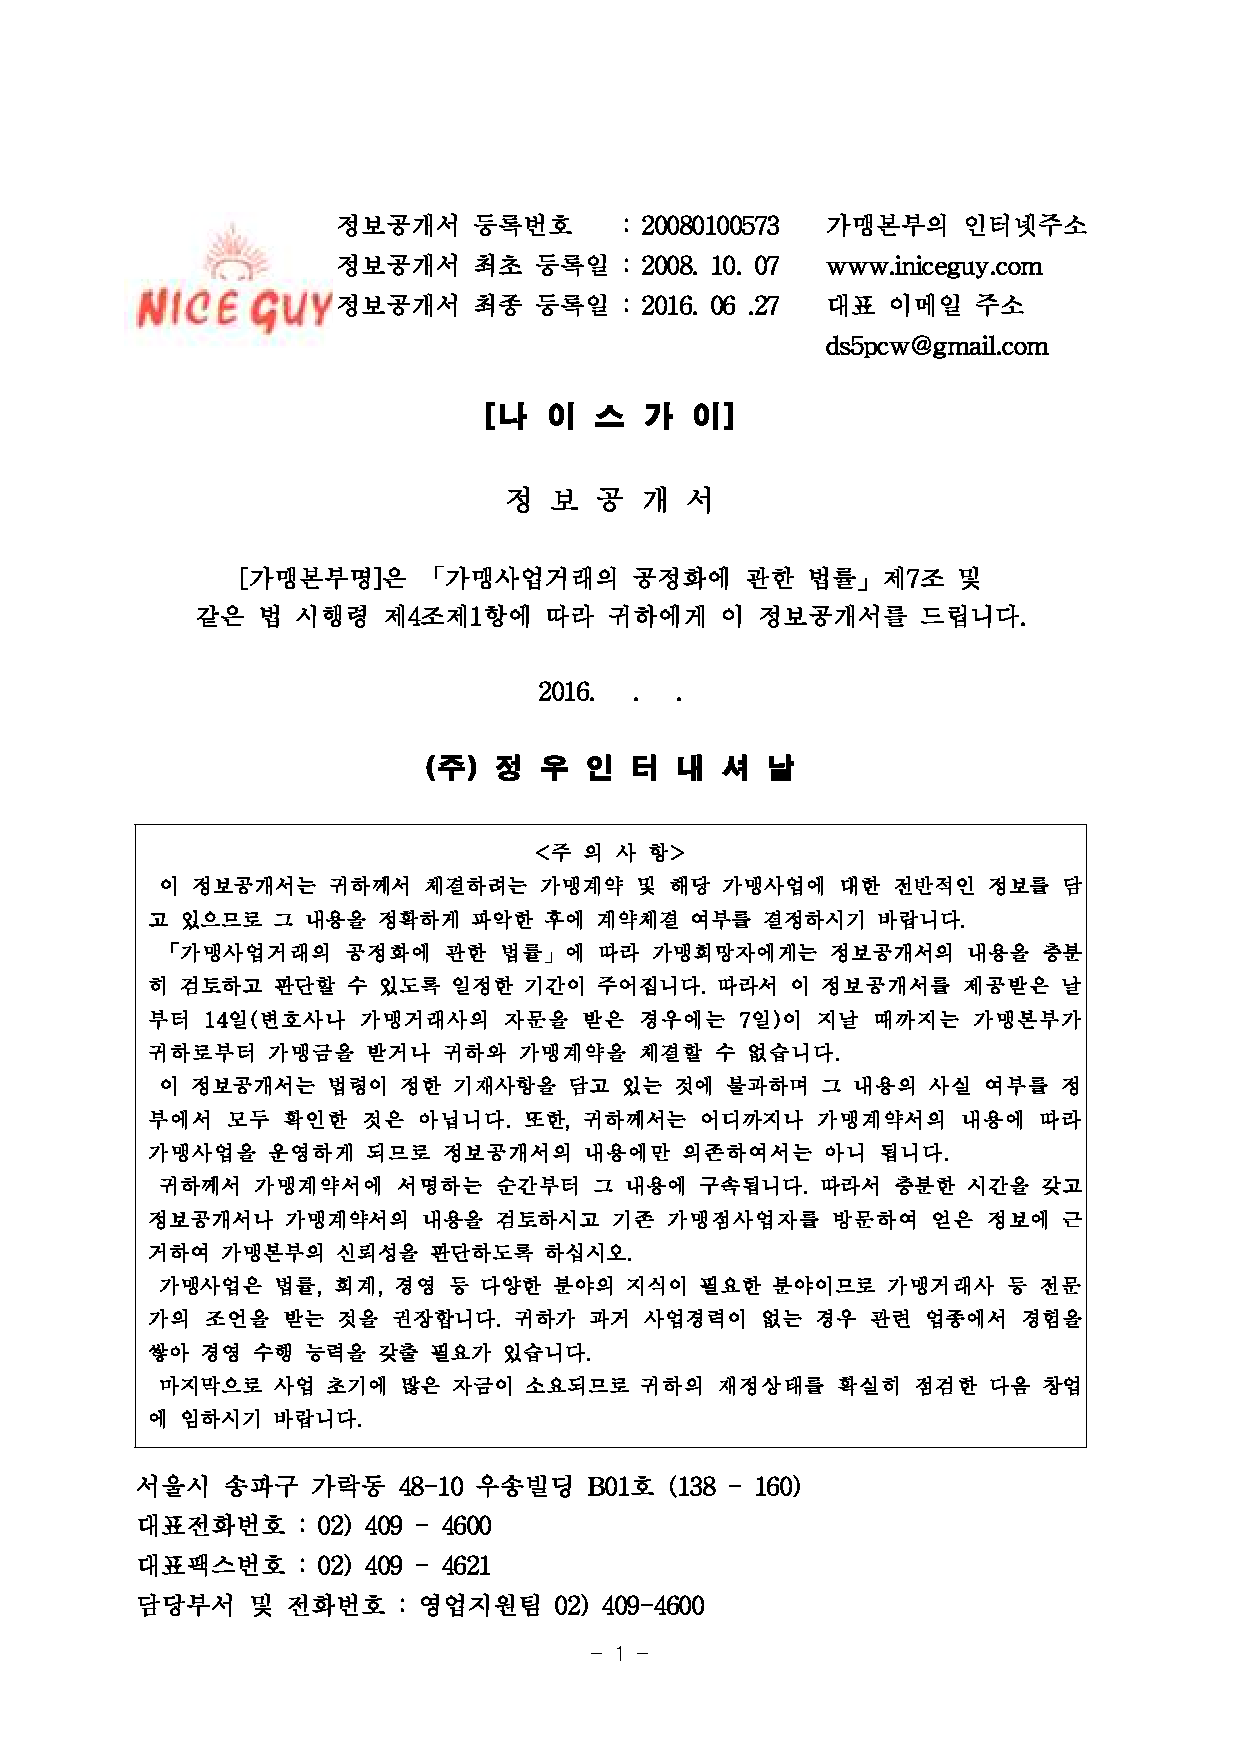
\includepdf[pages=1-45]{N.pdf}


































\end{document}
